\ifx\wholebook\relax \else
\documentclass[b5paper]{ctexart}
\usepackage[nomarginpar
  %, margin=.5in
]{geometry}

\addtolength{\oddsidemargin}{-0.05in}
\addtolength{\evensidemargin}{-0.05in}
\addtolength{\textwidth}{0.1in}
\usepackage[cn]{../../prelude}

\setcounter{page}{1}

\begin{document}

\title{快速排序和归并排序}

\author{刘新宇
\thanks{{\bfseries 刘新宇 } \newline
  Email: liuxinyu95@gmail.com \newline}
  }

\maketitle
\fi

\markboth{快速排序和归并排序}{基本算法}

\ifx\wholebook\relax
\chapter{快速排序和归并排序}
\numberwithin{Exercise}{chapter}
\fi

人们已证明,基于比较的排序算法的性能上限为$O(n \lg n)$\cite{TAOCP}。本章介绍两种分治排序算法:快速排序和归并排序,性能均可达到$O(n \lg n)$。我们还会介绍它们的若干变形,如自然归并排序,原地归并排序等。

\section{快速排序}
\index{快速排序}

\begin{figure}[htbp]
 \centering
 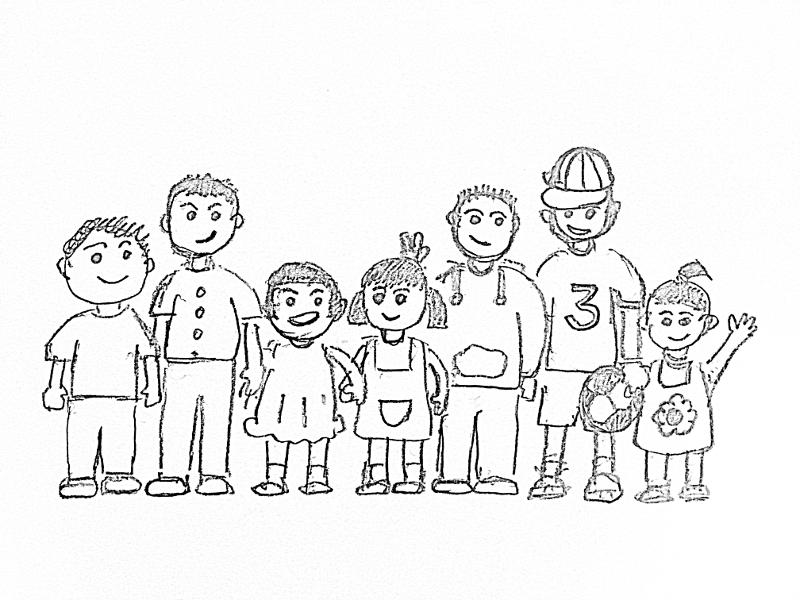
\includegraphics[scale=0.3]{img/kids}
 \captionsetup{labelformat=empty}
 %\caption{}
 \label{fig:knuth-ssort}
\end{figure}

考虑安排一组小朋友按照个头排队。

\begin{enumerate}
  \item 第一个小朋友举起手。所有比这个小朋友矮的都站到他的左侧去;所有比他高的站到他的右侧去;
  \item 所有站到左侧的小朋友重复这一步骤;站到右侧的也重复这一步骤。
\end{enumerate}

设孩子们的身高为(厘米):$[102, 100, 98, 95, 96, 99, 101, 97]$。表\cref{tab:kids-sort}描述了这一排队过程。第一步,身高为102厘米的孩子举手。我们称这个小朋友为基准,标以下划线。恰巧他的身高最高。所有人都站到他左侧,如表中第二行所示。此时,身高为102厘米的小朋友站到了最终应站的位置,我们标以引号。第二步,身高为100厘米的孩子举手。身高为98、95、96、99厘米的小朋友站到了他的左侧,而身高为101厘米的小朋友站到了右侧。如表中第三行。第三步,身高为98厘米的小朋友成为了左侧的基准;身高为101厘米的小朋友成为了右侧基准。但右侧那组只有一人,无需继续排序。重复同样的方法,直到所有人都站到最终位置。

\begin{table}[htbp]
\centering
\begin{tabular}{ | c c c c c c c c |}
\hline
\underline{102} & 100 & 98 & 95 & 96 & 99 & 101 & 97 \\
\underline{100} & 98 & 95 & 96 & 99 & 101 & 97 & `102' \\
\underline{98} & 95 & 96 & 99 & 97 & `100' & 101 & `102' \\
\underline{95} & 96 & 97 & `98' & 99 & `100' & `101' & `102' \\
`95' & \underline{96} & 97 & `98' & `99' & `100' & `101' & `102' \\
`95' & `96' & 97 & `98' & `99' & `100' & `101' & `102' \\
`95' & `96' & `97' & `98' & `99' & `100' & `101' & `102' \\
\hline
\end{tabular}
\caption{按身高排队过程}
\label{tab:kids-sort}
\end{table}

我们可以归纳出快速排序的定义。对序列$L$进行排序时:

\begin{itemize}
\item 若$L$为空$[\ ]$,则排序结果为空$[\ ]$;
\item 否则,在$L$中任选一个元素作为基准$p$,然后递归地将$L$中不大于$p$的元素排序,将结果置于$p$的左侧,\textbf{同时}将所有大于$p$的元素排序,结果置于右侧。
\end{itemize}

我们说“同时”而不是“然后”。左右两侧的递归排序是并行的。快速排序由霍尔(C. A. R. Hoare)在1960年提出\cite{TAOCP}、\cite{wiki-qs}。我们的定义中并没有说明如何选择基准。这里有多种可能,例如总选择第一个元素作为基准$p$:

\be
\begin{array}{rcl}
sort\ [\ ] & = & [\ ] \\
sort\ (x \cons xs) & = & sort\ [y | y \in xs, y \leq x] \doubleplus [x] \doubleplus sort\ [y | y \in xs, x < y] \\
\end{array}
\ee

我们使用了集合论中的“策梅罗——弗兰克尔”表达式(简称ZF表达式)的列表形式\footnote{以纪念对现代集合论创始人策梅罗(Zermelo)、弗兰克尔(Frankel)。}。一个ZF表达式$\{ a | a \in S, p_1(a), p_2(a), ... \}$表示从集合$S$中选取使得断言$p_1, p_2, ...$都为真的元素(见第一章)。如下面的例子代码:

\lstset{frame = single}
\begin{Haskell}
sort [] = []
sort (x:xs) = sort [y | y<-xs, y <= x] ++ [x] ++ sort [y | y<-xs, x < y]
\end{Haskell}

我们假设按非递减的顺序排序。也可以按照其它规则排序,以适于各种场景,如数字、字符串、或更复杂的内容。为此我们可以把比较条件抽象成参数(见第三章)。我们并不要求比较条件一定是全序,但是至少要满足\textbf{严格弱序}\cite{wiki-total-order}、\cite{wiki-sweak-order}(见第九章)。简单起见,我们仅考虑使用$\leq$作为比较条件。

\subsection{划分}
\index{快速排序!划分(partition)}
在基本快速排序的定义中,我们遍历了两次:第一次获得了所有$\leq x$的元素,第二次获得所有$> x$的元素。可以将它们合并成一次划分过程:

\be
\begin{array}{rcl}
\textit{part}\ p\ [\ ] & = & ([\ ], [\ ]) \\
\textit{part}\ p\ (x \cons xs) & = & \begin{cases}
 p(x): & (x \cons as, bs), \text{其中}: (as, bs) = \textit{part}\ p\ xs \\
 \text{否则}: & (as, x \cons bs) \\
\end{cases} \\
\end{array}
\ee

这样快速排序的定义变为:

\be
\begin{array}{rcl}
sort\ [\ ] & = & [\ ] \\
sort\ (x \cons xs) & = & sort\ as \doubleplus [x] \doubleplus sort\ bs, \text{其中}: (as, bs) = \textit{part}\ (\leq x)\ xs \\
\end{array}
\ee

我们也可以用叠加来定义划分:

\be
\textit{part}\ p\ = foldr\ f\ ([\ ], [\ ])
\ee

其中$f$定义为:

\be
f\ (as, bs)\ x = \begin{cases}
p(x): & (x \cons as, bs) \\
\text{否则}: & (as, x \cons bs) \\
\end{cases}
\ee

使用叠加实现的划分,本质上是向划分结果$(as, bs)$累积的过程。若$p(x)$,则累积$x$到$as$,否则累积到$bs$。这样我们可以实现一个尾递归的划分:

\be
\begin{array}{rcl}
\textit{part}\ p\ [\ ]\ as\ bs & = & (as, bs) \\
\textit{part}\ p\ (x \cons xs)\ as\ bs & = & \begin{cases}
  p(x): & \textit{part}\ p\ xs\ (x \cons as)\ bs \\
  \text{否则}: & \textit{part}\ p\ xs\ as\ (x \cons bs) \\
\end{cases}
\end{array}
\ee

下面的表达式对$x \cons xs$进行划分:

\[
(as, bs) = \textit{part}\ (\leq x)\ xs\ [\ ]\ [\ ]
\]

快速排序定义中的连接操作$sort\ as \doubleplus [x] \doubleplus sort\ bs$可以进一步转化为累积形式:

\be
\begin{array}{rcl}
sort\ s\ [\ ] & = & s \\
sort\ s\ (x \cons xs) & = & sort\ (x : sort\ s\ bs)\ as \\
\end{array}
\ee

其中$s$为累积结果。我们传入一个空列表来启动排序:$qsort = sort\ [\ ]$。划分完成时,需要递归地对两个子列表$as$、$bs$排序。我们可以先对$bs$排序,将$x$链接到结果前,作为新的“累积结果”传入后续的排序中。

\begin{Haskell}
sort = sort' []

sort' acc [] = acc
sort' acc (x:xs) = sort' (x : sort' acc bs) as where
  (as, bs) = part xs [] []
  part [] as bs = (as, bs)
  part (y:ys) as bs | y <= x = part ys (y:as) bs
                    | otherwise = part ys as (y:bs)
\end{Haskell}

\subsection{原地排序}
我们接下来考虑如何实现原地划分、排序。图\cref{fig:partition-1-way}描述了这种一次遍历划分的方法\cite{Bentley}\cite{CLRS}。我们从左向右扫描数组。任何时候,数组都由图\cref{fig:partition-1-way} (a)所示的几部分组成:

\begin{figure}[htbp]
   \centering
   \subcaptionbox{划分的不变性质}{
      \begin{tikzpicture}[scale=0.8]
      \draw (0, 0) rectangle (1, 1) node (xl) [pos=.5] {x[l]}
            (1, 0) rectangle (5, 1) node (leq) [pos=.5] {... $\leq p$ ...}
            (5, 0) rectangle (9, 1) node (ge) [pos=.5] {... $> p$ ...}
            (9, 0) rectangle (11, 1) node (rest) [pos=.5] {...?...}
            (11, 0) rectangle (12, 1) node (xu) [pos=.5] {x[u]};
      \fill [black] (5, 0) rectangle (5.1, 1) node (leftbar) [pos=.5] {}
                    (9, 0) rectangle (9.1, 1) node (rightbar) [pos=.5] {};
      \draw (0, 2) node (pivot) {$p = x[l]$}
            (5, 2) node (left) {左边界$L$}
            (9, 2) node (right) {右边界$R$};
      \draw[thick, ->] (pivot) edge (xl)
                       (left) edge [bend right] (leftbar)
                       (right) edge [bend right] (rightbar);
      \end{tikzpicture}} \\
   \subcaptionbox{开始}{
      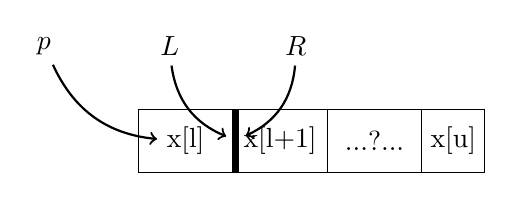
\begin{tikzpicture}[scale=0.8]
      \draw (-0.5, 0) rectangle (1, 1) node (xl) [pos=.5] {x[l]}
            (1, 0) rectangle (2.5, 1) node (xl1) [pos=.5] {x[l+1]}
            (2.5, 0) rectangle (4, 1) node (rest) [pos=.5] (ai) {...?...}
            (4, 0) rectangle (5, 1) node (xu) [pos=.5] {x[u]};
      \fill [black] (1, 0) rectangle (1.1, 1) node (leftbar) [pos=.5] {};
      \draw (-2, 2) node (pivot) {$p$}
            (0, 2) node (left) {$L$}
            (2, 2) node (right) {$R$};
      \draw[thick, ->] (pivot) edge [bend right] (xl)
                       (left) edge [bend right] (leftbar)
                       (right) edge [bend left] (leftbar);
      \end{tikzpicture}} \\
   \subcaptionbox{结束}{
      \begin{tikzpicture}[scale=0.8]
      \draw (0, 0) rectangle (1, 1) node (xl) [pos=.5] {x[l]}
            (1, 0) rectangle (5, 1) node (leq) [pos=.5] {... $\leq p$ ...}
            (5, 0) rectangle (6, 1) node (xleft) [pos=.5] {x[$L$] }
            (6, 0) rectangle (10, 1) node (ge) [pos=.5] {... $> p$ ...}
            (10, 0) rectangle (11, 1) node (xu) [pos=.5] {x[u]};
      \fill [black] (6, 0) rectangle (6.1, 1) node (leftbar) [pos=.5] {}
                    (11, 0) rectangle (11.1, 1) node (rightbar) [pos=.5] {};
      \draw (0, 2) node (pivot) {$p$}
            (6, 2) node (left) {$L$}
            (12, 2) node (right) {$R$};
      \draw[thick, ->] (pivot) edge (xl)
                       (left) edge [bend right] (leftbar)
                       (right) edge [bend left] (rightbar);
      \draw[thick, <->] (xl) edge [bend right] node [below] {交换} (xleft);
      \end{tikzpicture}} \\
   \caption{用首个元素作基准$p$划分一段数组}
   \label{fig:partition-1-way}
\end{figure}

\begin{itemize}
\item 最左侧为基准$p$。划分结束时,$p$被移动到最终位置;
\item 一段只包含$\leq p$的部分。这一段的右侧边界为$L$;
\item 一段只包含$> p$的部分。这一段的右侧边界为$R$。$L$、$R$之间的元素都大于$p$;
\item $R$后面的元素尚未处理。这部分的元素可能大于或不大于$p$。
\end{itemize}

划分开始时,$L$指向$p$,$R$指向$p$的下一个元素,如图\cref{fig:partition-1-way} (b)所示。然后不断向右移动$R$进行处理,直到$R$越过数组右侧。每次迭代,都比较$R$指向的元素和$p$。若$x[R] > p$,它应位于$L$和$R$之间,我们继续向前移动$R$;否则$x[R] \leq p$,它应该位于$L$左侧。我们将$L$向前移动一步,然后交换$x[L]$和$x[R]$。当$R$越过最后一个位置时,所有的元素都已处理完。$> p$的元素都被移动到了$L$右侧,而其它元素位于$L$左侧。此时我们需要移动$p$,使它位于这两段的中间。为此,我们交换$p$和$x[L]$。如图\cref{fig:partition-1-way} (c)中的双向箭头所示。$L$最终指向$p$,将整个数组分成两部分。我们将$L$作为划分的结果返回。为了方便后继处理,我们将$L$增加1,使得它指向第一个大于$p$的元素。令数组为$A$,待划分区间的上下界为$l, u$,原地划分实现如下:

\begin{algorithmic}[1]
\Function{Partition}{A, l, u}
  \State $p \gets A[l]$  \Comment{基准}
  \State $L \gets l$ \Comment{左侧}
  \For{$R$ in $[l+1, u]$} \Comment{对右侧迭代}
    \If{$p \geq A[R]$}
      \State $L \gets L + 1$
      \State \textproc{Exchange} $A[L] \leftrightarrow A[R]$
    \EndIf
  \EndFor
  \State \textproc{Exchange} $A[L] \leftrightarrow p$
  \State \Return $L + 1$ \Comment{返回划分的位置}
\EndFunction
\end{algorithmic}

表\cref{tab:partition-steps}给出了划分数组$[3, 2, 5, 4, 0, 1, 6, 7]$的步骤。

\begin{table}[htbp]
\centering
\begin{tabular}{|llllllll|l|}
\hline
\underline{3}(l)  & 2(r) & 5 & 4 & 0 & 1 & 6 & 7 & 开始,$p = 3$、$l = 1$、$r = 2$ \\
\underline{3} & 2(l)(r) & 5 & 4 & 0 & 1 & 6 & 7 & $2 < 3$,移动$l$($r=l$)\\
\underline{3} & 2(l) & 5(r) & 4 & 0 & 1 & 6 & 7 & $5 > 3$, 继续 \\
\underline{3} & 2(l) & 5 & 4(r) & 0 & 1 & 6 & 7 & $4 > 3$, 继续 \\
\underline{3} & 2(l) & 5 & 4 & 0(r) & 1 & 6 & 7 & $0 < 3$ \\
\underline{3} & 2 & 0(l) & 4 & 5(r) & 1 & 6 & 7 & 移动$l$,然后和$r$交换 \\
\underline{3} & 2 & 0(l) & 4 & 5 & 1(r) & 6 & 7 & $1 < 3$ \\
\underline{3} & 2 & 0 & 1(l) & 5 & 4(r) & 6 & 7 & 移动$l$,然后和$r$交换 \\
\underline{3} & 2 & 0 & 1(l) & 5 & 4 & 6(r) & 7 & $6 > 3$,继续 \\
\underline{3} & 2 & 0 & 1(l) & 5 & 4 & 6 & 7(r) & $7 > 3$,继续 \\
1 & 2 & 0 & 3 & 5(l+1) & 4 & 6 & 7 & $r$越过了边界,交换$p$和$l$ \\
\hline
\end{tabular}
\caption{扫描并划分数组} \label{tab:partition-steps}
\end{table}

使用\textproc{Partition},可以实现快速排序如下:

\begin{algorithmic}[1]
\Procedure{Quick-Sort}{$A, l, u$}
  \If{$l < u$}
    \State $m \gets$ \Call{Partition}{$A, l, u$}
    \State \Call{Quick-Sort}{$A, l, m - 1$}
    \State \Call{Quick-Sort}{$A, m, u$}
  \EndIf
\EndProcedure
\end{algorithmic}

我们在排序时传入数组上下界,如:\textproc{Quick-Sort}($A, 1, |A|$)。如果数组片段为空或只含有一个元素,我们直接返回。

\begin{Exercise}\label{ex:basic-qsort}
\Question{改进基本快速排序的定义,除了列表为空外,优化对单元素列表的处理。}
\end{Exercise}

\begin{Answer}[ref = {ex:basic-qsort}]
\Question{改进基本快速排序的定义,除了列表为空外,优化对单元素列表的处理。
增加一条处理
\begin{Haskell}
sort [x] = [x]
\end{Haskell}
}
\end{Answer}

\subsection{性能分析}
\index{快速排序!性能分析}

快速排序在实际应用中性能良好。我们需要使用统计学工具来分析平均情况下的性能。首先分析最好和最坏情况。最好情况下,每次划分都将序列均分。如图\cref{fig:qsort-best}所示,共需要$O(\lg n)$次递归调用。第一层划分一次,处理$n$个元素;第二层划分两次,每次处理$n/2$个元素,总体执行时间为$2 O(n/2) = O(n)$。第三层划分四次,每次处理$n/4$个元素,总体执行时间也是$O(n)$……最后一层总共有$n$个片段,每个片段一个元素,总时间也是$O(n)$。将所有层的执行时间相加,得到快速排序在最好情况下的性能为$O(n \lg n)$。

\begin{figure}[htbp]
 \centering
 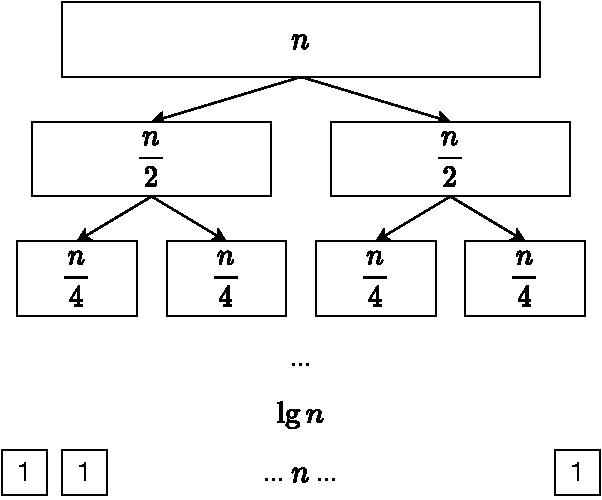
\includegraphics[scale=0.55]{img/qsort-best}
 \caption{最好情况,每次均分。}
 \label{fig:qsort-best}
\end{figure}

最坏情况下,划分极不平衡。一部分长$O(1)$,另一部分的长$O(n)$。递归的深度退化为$O(n)$。最好情况下,快速排序过程形成一棵平衡二叉树;最坏情况下,形成一棵极不平衡的树,每个节点都只有一棵子树,另一棵子树为空。二叉树退化成了一个长度为$O(n)$的链表。而在每一层中,所有的元素都被处理,因此最坏情况下的性能为$O(n^2)$,这和插入排序、选择排序的性能相当。我们可以考虑几种特殊的最坏情况,例如大量元素都相等导致划分结果不平衡。另外已序序列也导致不平衡划分。还有其它一些情况导致性能下降,不存在一种方法可以完全避免最坏情况。

\subsubsection{平均情况\texorpdfstring{$\bigstar$}{★}}
\index{快速排序!平均情况分析}

快速排序在平均情况下性能良好。即使每次划分总得到长度比为1:9的两部分,性能仍然为$O(n \lg n)$\cite{CLRS}。我们给出两种方法分析快速排序在平均情况下的复杂度。第一种方法利用比较操作的次数来考量性能\cite{CLRS}。在选择排序中,任何两个元素都进行了比较。快速排序避免了很多不必要的比较。考虑划分列表$[a_1, a_2, a_3, ..., a_n]$,选择$a_1$作为基准,划分结果产生两个子列表$A = [x_1, x_2, ..., x_k]$和$B = [y_1, y_2, ..., y_{n-k-1}]$。在后继的排序过程中,$A$中任何元素都不再和$B$中的任何元素进行比较。令最终排序的结果为$[a_1, a_2, ..., a_n]$,我们有:若$a_i < a_j$,当且仅当存在某一元素$a_k$满足$a_i < a_k < a_j$,并且$a_k$在$a_i$或$a_j$之前被选为基准时,我们不再对$a_i$和$a_j$进行比较。也就是说,若$a_i$与$a_j$进行比较,则要么$a_i$、要么$a_j$一定在所有$a_{i+1} < a_{i+2} < ... < a_{j-1}$之前被选为基准。令$P(i, j)$代表$a_i$和$a_j$进行比较的概率,我们有:

\be
P(i, j) = \frac{2}{j - i + 1}
\ee

全部比较操作的总数可以这样得到:

\be
C(n) = \sum_{i=1}^{n-1}\sum_{j=i+1}^{n} P(i, j)
\ee

如果我们比较了$a_i$和$a_j$,在接下来的快速排序中,就不再比较$a_j$和$a_i$,并且元素$a_i$永远不会和自己进行比较。因此在上式中,$i$的上限为$n-1$,$j$的下限为$i+1$。将概率代入得:

\be
\begin{array}{rl}
C(n) & = \displaystyle \sum_{i=1}^{n-1}\sum_{j = i+1}^{n} \frac{2}{j - i + 1} \\
     & = \displaystyle \sum_{i=1}^{n-1}\sum_{k=1}^{n-i} \frac{2}{k+1} \\
\end{array}
\ee

使用调和级数\cite{wiki-harmonic}。

\[
H_n = 1 + \frac{1}{2} + \frac{1}{3} + .... = \ln n + \gamma + \epsilon_n
\]

因此:

\be
C(n) = \sum_{i=1}^{n-1} O(\lg n) = O(n \lg n)
\ee

第二种分析方法利用递归。令列表长度$n$,划分后得到两个长度为$i$和$n-i-1$的部分。划分过程比较基准$p$和每个元素,它自身用时$cn$。我们有如下递归关系:

\be
T(n) = T(i) + T(n-i-1) + c n
\ee

其中$T(n)$是对长度为$n$的列表进行快速排序所用的时间。$i$以相同的概率在$0, 1, ..., n-1$中取值。对上述等式取数学期望:

\be
\renewcommand*{\arraystretch}{1.5}
\begin{array}{rl}
T(n) & = E(T(i)) + E(T(n-i-1)) + c n \\
     & = \displaystyle \frac{1}{n} \sum_{i=0}^{n-1}T(i) + \frac{1}{n} \sum_{i=0}^{n-1}T(n-i-1) + cn \\
     & = \displaystyle \frac{1}{n} \sum_{i=0}^{n-1}T(i) + \frac{1}{n} \sum_{j=0}^{n-1}T(j) + cn \\
     & = \displaystyle \frac{2}{n} \sum_{i=0}^{b-1}T(i) + cn
\end{array}
\ee

两边同时乘以$n$:

\be
n T(n) = 2 \sum_{i=0}^{n-1} T(i) + c n^2
\label{eq:ntn}
\ee

将$n$用$n-1$替换,得到另一等式:

\be
(n-1) T(n-1) = 2 \sum_{i=0}^{n-2} T(i) + c (n-1)^2
\label{eq:n1tn1}
\ee

用式(\cref{eq:ntn})减去式(\cref{eq:n1tn1})消去所有的$T(i)$,其中$0 \leq i < n-1$。

\be
n T(n) = (n + 1) T(n-1) + 2cn - c
\ee

忽略常数$c$,上式简化为:

\be
\frac{T(n)}{n+1} = \frac{T(n-1)}{n} + \frac{2c}{n+1}
\ee

依次代入$n-1$、$n-2$……得到$n-1$个等式。

\[
\frac{T(n-1)}{n} = \frac{T(n-2)}{n-1} + \frac{2c}{n}
\]

\[
\frac{T(n-2)}{n-1} = \frac{T(n-3)}{n-2} + \frac{2c}{n-1}
\]

\[
...
\]

\[
\frac{T(2)}{3} = \frac{T(1)}{2} + \frac{2c}{3}
\]

将所有等式相加,消去左右相同的部分,化简得到一个关于$n$的函数。

\be
\frac{T(n)}{n+1} = \frac{T(1)}{2} + 2c \sum_{k=3}^{n+1} \frac{1}{k}
\ee

利用调和级数,最终的结果为:

\be
O(\frac{T(n)}{n+1}) = O(\frac{T(1)}{2} + 2c \ln n + \gamma + \epsilon_n) = O(\lg n)
\ee

因此

\be
O(T(n)) = O(n \lg n)
\ee

\subsection{改进}
\index{快速排序!改进} \index{快速排序!三分划分}

快速排序性能优异,但在最坏情况下,性能会退化到平方级别。如果数据随机分布,出现最坏情况的概率很低。尽管如此,工程上常常采用一些方法以避免或减少出现最坏情况。我们给出的划分实现\textproc{Partition}在处理大量重复元素时出现性能下降。考虑含有$n$个相等元素的特殊序列$[x, x, ..., x]$:

\begin{enumerate}
\item 基本快速排序:任选一个元素作为基准$p = x$,分割后得到两个序列:$[x, x, ..., x]$,长度为$n-1$,另外一个序列为空。接下来递归地对长为$n-1$的序列排序。总复杂度为$O(n^2)$。
\item 只用严格的$< x$、$> x$进行划分。结果是两个空序列和$n$个等于$x$的元素。接下来的递归只应用到两个空列上并立即结束。结果为$[\ ] \doubleplus [x, x, ..., x] \doubleplus [\ ]$。总复杂度为$O(n)$。
\end{enumerate}

据此,我们对划分进行改进:相对于二分划分,\textbf{三分划分}能更好地处理重复元素。

\be
\begin{array}{rcl}
sort\ [\ ] & = & [\ ] \\
sort\ (x \cons xs) & = & sort\ S \doubleplus sort\ E \doubleplus sort\ G
\end{array}
\ee

其中:

\[
\begin{cases}
S = [ y | y \in xs, y < x ] \\
E = [ y | y \in xs, y = x ] \\
G = [ y | y \in xs, y > x ] \\
\end{cases}
\]

这一实现需要线性时间将三个子列表连接起来。我们可以使用一个累积变量进行改进:$qsort = sort\ [\ ]$。其中:

\be
\begin{array}{rcl}
sort\ A\ [\ ] & = & A \\
sort\ A\ (x \cons xs) & = & sort\ (E \doubleplus sort\ A\ G)\ S \\
\end{array}
\ee

我们将非空列表划分为三个子列表$S, E, G$,其中$E$中元素全相等,无需进一步排序。我们先使用累积变量$A$对$G$排序,将结果连接到$E$的后面,作为新的累积变量再对$S$排序。划分也可以使用累积变量改进:

\be
\begin{array}{rcl}
part\ S\ E\ G\ x\ [\ ] & = & (S, E, G) \\
part\ S\ E\ G\ x\ (y \cons ys) & = & \begin{cases}
  y < x: & (y \cons S, E, G) \\
  y = x: & (S, y \cons E, G) \\
  y > x: & (S, E, y \cons G) \\
  \end{cases} \\
\end{array}
\ee

理查德$\cdot$伯德给出了另一种改进\cite{fp-pearls},它不立即连接递归排序的结果,而是把排好的子列表保存起来,最终再连接在一起:

\begin{Haskell}
sort :: (Ord a) => [a] -> [a]
sort = concat . (pass [])

pass xss [] = xss
pass xss (x:xs) = step xs [] [x] [] xss where
    step [] as bs cs xss = pass (bs : pass xss cs) as
    step (x':xs') as bs cs xss | x' <  x = step xs' (x':as) bs cs xss
                               | x' == x = step xs' as (x':bs) cs xss
                               | x' >  x = step xs' as bs (x':cs) xss
\end{Haskell}

\index{快速排序!双向扫描}
罗伯特$\cdot$塞奇维克(Robert Sedgewick)给出了\textbf{双向扫描}的划分方法\cite{qsort-impl}\cite{Bentley}。使用两个指针$i, j$从左右两侧相向扫描。开始时$i, j$指向数组左右边界,选择最左侧的元素作为基准$p$。然后左指针$i$向右扫描直到遇到一个$\geq p$的元素;另外\footnote{两轮扫描可以并发。}右指针$j$向左扫描直到遇到一个$\leq p$的元素。此时,所有$i$左边的元素都$< p$,所有$j$右边的元素都$> p$。$i$指向一个$\geq p$的元素,而$j$指向一个$\leq p$的元素。如图\cref{fig:partition-2-way} (a)。为了将全部$\leq p$的元素划分到左侧,其余元素划分到右侧,我们交换$i$和$j$指向的两个元素。然后恢复扫描,重复上面的步骤直到$i$和$j$相遇或者交错。在划分的任何时刻,总保持着不变条件:所有$i$左侧的元素(包括$i$)都$\leq p$;所有$j$右侧的元素(包括$j$)都$\geq p$。$i$和$j$之间的元素尚未处理。如图\cref{fig:partition-2-way} (b)。

\begin{figure}[htbp]
   \centering
   \subcaptionbox{指针$i$和$j$停止前进时}{
      \begin{tikzpicture}[scale=0.8]
      \draw (0, 0) rectangle (1, 1) node (xl) [pos=.5] {x[l]}
            (1, 0) rectangle (5, 1) node (leq) [pos=.5] {... $< p$ ...}
            (5, 0) rectangle (6, 1) node (xi) [pos=.5] {x[i]}
            (6, 0) rectangle (8, 1) node (rest) [pos=.5] {... ? ...}
            (8, 0) rectangle (9, 1) node (xj) [pos=.5] {x[j]}
            (9, 0) rectangle (13, 1) node (ge) [pos=.5] {... $> p$ ...};
      \draw (0, 2) node (pivot) {基准$p$}
            (5, 2) node (left) {$\geq p$}
            (8, 2) node (right) {$\leq p$};
      \draw[thick, ->] (pivot) edge (xl)
                       (left) edge [bend right] (xi)
                       (right) edge [bend right] (xj);
      \end{tikzpicture}} \\
   \subcaptionbox{划分不变条件}{
      \begin{tikzpicture}[scale=0.8]
      \draw (0, 0) rectangle (1, 1) node (xl) [pos=.5] {x[l]}
            (1, 0) rectangle (5, 1) node (leq) [pos=.5] {... $\leq p$ ...}
            (5, 0) rectangle (7, 1) node (rest) [pos=.5] {... ? ...}
            (7, 0) rectangle (11, 1) node (ge) [pos=.5] {... $\geq p$ ...};
      \fill [black] (5, 0) rectangle (5.1, 1) node (ibar) [pos=.5] {}
                    (7, 0) rectangle (7.1, 1) node (jbar) [pos=.5] {};
      \draw (0, 2) node (pivot) {基准$p$}
            (5, 2) node (i) {$i$}
            (7, 2) node (j) {$j$};
      \draw[thick, ->] (pivot) edge (xl)
                       (i) edge [bend right] (ibar)
                       (j) edge [bend right] (jbar);
      \end{tikzpicture}} \\
   \caption{双向扫描}
   \label{fig:partition-2-way}
\end{figure}

当$i$、$j$相遇或交错时,我们需要一次额外的交换,将最左侧的基准$p$交换到$j$指向的位置上。然后,我们对划分区间下界$l$和$j$之间的数组片段$A[l ... j)$;$i$和划分区间上界$u$之间的片段$A[i ... u)$进行递归排序。

\begin{algorithmic}[1]
\Procedure{Sort}{$A, l, u$} \Comment{排序区间:$[l, u)$}
  \If{$u - l > 1$} \Comment{包含1个以上的元素}
    \State $i \gets l$, $j \gets u$
    \State $p \gets A[l]$ \Comment{基准}
    \Loop
      \Repeat
        \State $i \gets i + 1$
      \Until{$A[i] \geq p$} \Comment{忽略$i \geq u$的情况}
      \Repeat
        \State $j \gets j - 1$
      \Until{$A[j] \leq p$} \Comment{忽略$j < l$的情况}
      \If{$j < i$}
        \State break
      \EndIf
      \State \textproc{Exchange} $A[i] \leftrightarrow A[j]$
    \EndLoop
    \State \textproc{Exchange} $A[l] \leftrightarrow A[j]$ \Comment{移动$p$}
    \State \Call{Sort}{$A, l, j$}
    \State \Call{Sort}{$A, i, u$}
  \EndIf
\EndProcedure
\end{algorithmic}

\index{快速排序!三路划分}
考虑所有元素都相等的极端情况:数组划分为两段长度相等的子数组,发生了$\dfrac{n}{2}$次交换。由于划分是平衡的,所以总体性能仍然为$O(n \lg n)$,而没有退化。和此前的划分实现对比,这一方法的交换次数更少。它跳过了那些在基准正确一侧的元素不进行处理。我们可以把双向扫描和三路划分结合起来。只对不等于基准的元素进行递归。Jon Bentley和Douglas McIlroy给出了一个方法:如图\cref{fig:partition-3-way} (a)所示,先把所有和基准相等的元素保存在两侧\cite{3-way-part}\cite{opt-qs}。

\begin{figure}[htbp]
   \centering
   \subcaptionbox{三路划分的不变条件。}{
      \begin{tikzpicture}[scale=0.8]
      \draw (0, 0) rectangle (1, 1) node (xl) [pos=.5] {$x[l]$}
            (1, 0) rectangle (3, 1) node [pos=.5] {... $=$ ...}
            (3, 0) rectangle (5, 1) node [pos=.5] {... $<$ ...}
            (5, 0) rectangle (7, 1) node [pos=.5] {... ? ...}
            (7, 0) rectangle (9, 1) node [pos=.5] {... $>$ ...}
            (9, 0) rectangle (11, 1) node [pos=.5] {... $=$ ...};
      \fill [black] (3, 0) rectangle (3.1, 1) node (pbar) [pos=.5] {}
                    (5, 0) rectangle (5.1, 1) node (ibar) [pos=.5] {}
                    (7, 0) rectangle (7.1, 1) node (jbar) [pos=.5] {}
                    (9, 0) rectangle (9.1, 1) node (qbar) [pos=.5] {};
      \draw (0, 2) node (pivot) {基准}
            (3, 2) node (p) {$p$}
            (5, 2) node (i) {$i$}
            (7, 2) node (j) {$j$}
            (9, 2) node (q) {$q$};
      \draw[thick, ->] (pivot) edge (xl)
                       (p) edge [bend right] (pbar)
                       (i) edge [bend right] (ibar)
                       (j) edge [bend left] (jbar)
                       (q) edge [bend left] (qbar);
      \end{tikzpicture}} \\
   \subcaptionbox{将等于基准的元素交换到中间。}{\hspace{0.1\textwidth}
      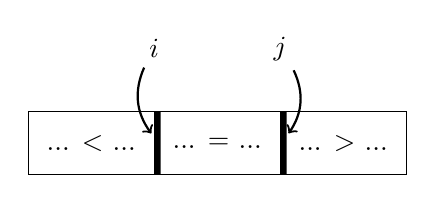
\begin{tikzpicture}[scale=0.8]
      \draw (0, 0) rectangle (2, 1) node [pos=.5] {... $<$ ...}
            (2, 0) rectangle (4, 1) node [pos=.5] {... $=$ ...}
            (4, 0) rectangle (6, 1) node [pos=.5] {... $>$ ...};
      \fill [black] (2, 0) rectangle (2.1, 1) node (ibar) [pos=.5] {}
                    (4, 0) rectangle (4.1, 1) node (jbar) [pos=.5] {};
      \draw (2, 2) node (i) {$i$}
            (4, 2) node (j) {$j$};
      \draw[thick, ->] (i) edge [bend right] (ibar)
                       (j) edge [bend left] (jbar);
      \end{tikzpicture}
      \hspace{0.1\textwidth}}
   \caption{三路划分}
   \label{fig:partition-3-way}
\end{figure}

扫描过程仍然是左右相向的。直到$i$遇到$\geq$基准的元素,并且$j$遇到$\leq$基准的元素。此时如果$i$和$j$没有相遇或者交错,我们不仅交换$A[i] \leftrightarrow A[j]$,同时检查$A[i], A[j]$是否等于基准。如果相等,就交换$A[i] \leftrightarrow A[p]$或$A[j] \leftrightarrow A[q]$。在划分结束前,我们需要把所有等于基准的元素从左右交换到中间。交换次数取决于重复元素的个数。如果所有元素唯一,则交换次数为零,不产生任何额外消耗。划分结果如图\cref{fig:partition-3-way} (b)所示。此后,我们只需要对“严格小于”和“严格大于”部分递归。

\begin{algorithmic}[1]
\Procedure{Sort}{$A, l, u$}
  \If{$u - l > 1$}
    \State $i \gets l$, $j \gets u$
    \State $p \gets l$, $q \gets u$ \Comment{指向相等元素的边界}
    \State $pivot \gets A[l]$
    \Loop
      \Repeat
        \State $i \gets i + 1$
      \Until{$A[i] \geq pivot$} \Comment{忽略$i \geq u$的错误处理}
      \Repeat
        \State $j \gets j - 1$
      \Until{$A[j] \leq pivot$} \Comment{忽略$j < l$的错误处理}
      \If{$j \leq i$}
        \State break
      \EndIf
      \State \textproc{Exchange} $A[i] \leftrightarrow A[j]$
      \If{$A[i] = pivot$} \Comment{处理相等的元素}
        \State $p \gets p + 1$
        \State \textproc{Exchange} $A[p] \leftrightarrow A[i]$
      \EndIf
      \If{$A[j] = pivot$}
        \State $q \gets q - 1$
        \State \textproc{Exchange} $A[q] \leftrightarrow A[j]$
      \EndIf
    \EndLoop
    \If{$i = j$ 且 $A[i] = pivot$}
      \State $j \gets j - 1$, $i \gets i + 1$
    \EndIf
    \For{$k$ from $l$ to $p$} \Comment{将相等的元素交换到中间}
      \State \textproc{Exchange} $A[k] \leftrightarrow A[j]$
      \State $j \gets j - 1$
    \EndFor
    \For{$k$ from $u-1$ down-to $q$}
      \State \textproc{Exchange} $A[k] \leftrightarrow A[i]$
      \State $i \gets i + 1$
    \EndFor
    \State \Call{Sort}{$A, l, j + 1$}
    \State \Call{Sort}{$A, i, u$}
  \EndIf
\EndProcedure
\end{algorithmic}

双向扫描加三路划分的逻辑变得复杂了,需要仔细处理各种边界条件。此前的单向扫描具有简单、直观的特点。我们考虑直接对它进行改进。首先需要调整不变条件。选择第一个元素作为基准$p$,如图\cref{fig:partition-3-way-lomuto}所示。任何时刻,左侧片段包含$< p$的元素;接下来的片段包含$= p$的元素;最右侧片段包含$> p$的元素。三个片段的边界分别为$i$、$k$、$j$。$[k, j)$之间是尚未扫描的元素。我们从左向右逐一扫描。开始时,$< p$的部分为空;$= p$的部分只有一个元素。$i$指向数组的下界,$k$指向$i$的下一个元素。$> p$的部分也为空,$j$指向数组上界。

\begin{figure}[htbp]
   \centering
      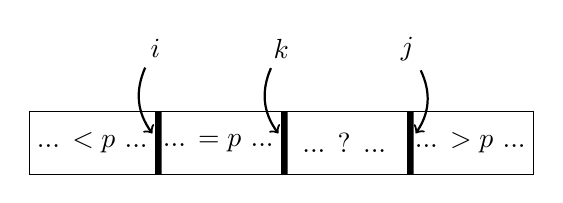
\begin{tikzpicture}[scale=0.8]
      \draw (0, 0) rectangle (2, 1) node [pos=.5] {... $< p$ ...}
            (2, 0) rectangle (4, 1) node [pos=.5] {... $= p$ ...}
            (4, 0) rectangle (6, 1) node [pos=.5] {... ? ...}
            (6, 0) rectangle (8, 1) node [pos=.5] {... $> p$ ...};
      \fill [black] (2, 0) rectangle (2.1, 1) node (ibar) [pos=.5] {}
                    (4, 0) rectangle (4.1, 1) node (kbar) [pos=.5] {}
                    (6, 0) rectangle (6.1, 1) node (jbar) [pos=.5] {};
      \draw (2, 2) node (i) {$i$}
            (4, 2) node (k) {$k$}
            (6, 2) node (j) {$j$};
      \draw[thick, ->] (i) edge [bend right] (ibar)
                       (k) edge [bend right] (kbar)
                       (j) edge [bend left] (jbar);
      \end{tikzpicture}
   \caption{单向扫描三路划分}
   \label{fig:partition-3-way-lomuto}
\end{figure}

划分开始后,我们逐一检查$k$指向的元素。如果它等于$p$,就移动$k$指向下一个元素;如果$> p$,我们将$A[k]$和未处理区间的最后一个元素$A[j-1]$交换,这样$> p$的区间长度就增加一。它的边界$j$向左移动一步。由于不确定移动到位置$k$的元素是否仍然大于$p$,我们需要再次比较,重复上述过程。否则,如果元素$< p$,我们将$A[k]$和$= p$的区间的第一个元素$A[i]$交换。当$k$和$j$相遇时,划分过程结束。

\begin{algorithmic}[1]
\Procedure{Sort}{$A, l, u$}
  \If{$u - l > 1$}
    \State $i \gets l$, $j \gets u$, $k \gets l + 1$
    \State $pivot \gets A[i]$
    \While{$k < j$}
      \While{$pivot < A[k]$}
        \State $j \gets j - 1$
        \State \textproc{Exchange} $A[k] \leftrightarrow A[j]$
      \EndWhile
      \If{$A[k] < pivot$}
        \State \textproc{Exchange} $A[k] \leftrightarrow A[i]$
        \State $i \gets i + 1$
      \EndIf
      \State $k \gets k + 1$
    \EndWhile
    \State \Call{Sort}{$A, l, i$}
    \State \Call{Sort}{$A, j, u$}
  \EndIf
\EndProcedure
\end{algorithmic}

和双向扫描加三路划分相比,这一实现相对简单但需要更多的交换次数。

\subsubsection{最差情况}

虽然三路划分能较好地应对大量重复元素,但仍然无法有效解决一些最差情况。例如,序列中的大部分元素已序时(无论是升序还是降序),划分结果不平衡。图\cref{fig:worst-cases-1}是两种极端情况:$[x_1 < x_2 < ... < x_n]$和$[y_1 > y_2 > ... > y_n]$的划分结果。我们可以给出更多的最差情况,例如$[x_m, x_{m-1}, ..., x_2, x_1, x_{m+1}, x_{m+2}, ... x_n]$,其中$[ x_1 < x_2 < ... < x_n]$,以及$[x_n, x_1, x_{n-1}, x_2, ... ]$。如图\cref{fig:worst-cases-2}所示。

\begin{figure}[htbp]
   \centering
   \subcaptionbox{$[x_1 < x_2 < ... < x_n]$的划分树。$\leq p$的部分总为空。}{\hspace{.3\textwidth} 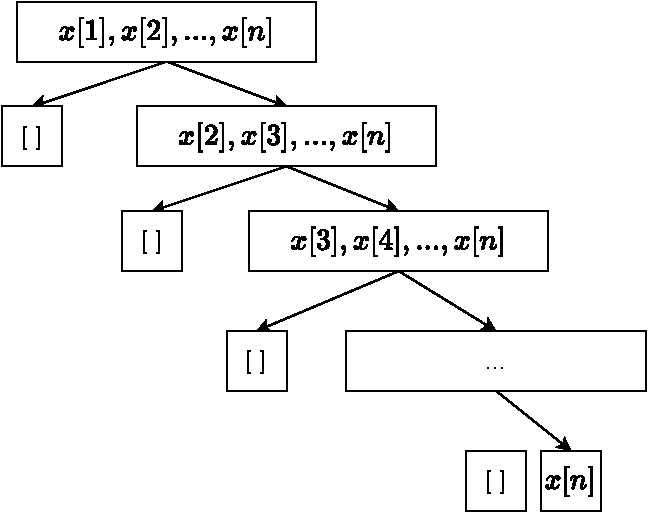
\includegraphics[scale=0.5]{img/unbalanced} \hspace{.3\textwidth}} \\
   \subcaptionbox{$[y_1 > y_2 > ... > y_n]$的划分树,$\geq p$的部分总为空。}{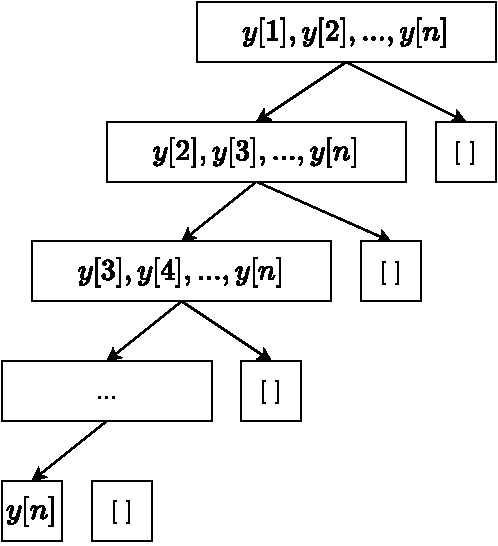
\includegraphics[scale=0.5]{img/unbalanced-2}} \\
   \caption{两种最差情况}
   \label{fig:worst-cases-1}
\end{figure}

\begin{figure}[htbp]
   \centering
   \subcaptionbox{除了第一次划分,其它都不平衡。}{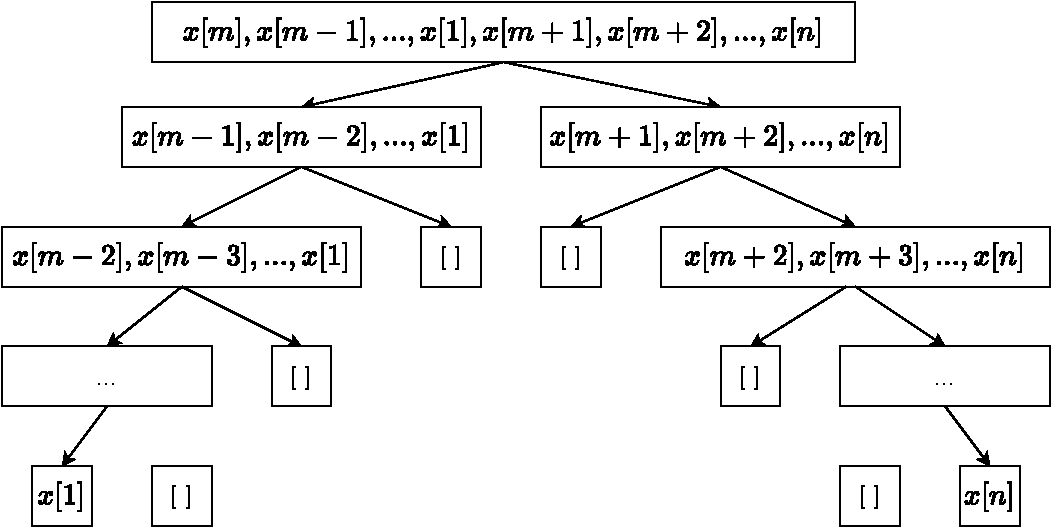
\includegraphics[scale=0.4]{img/unbalanced-3}} \\
   \subcaptionbox{一个之字形的划分树。}{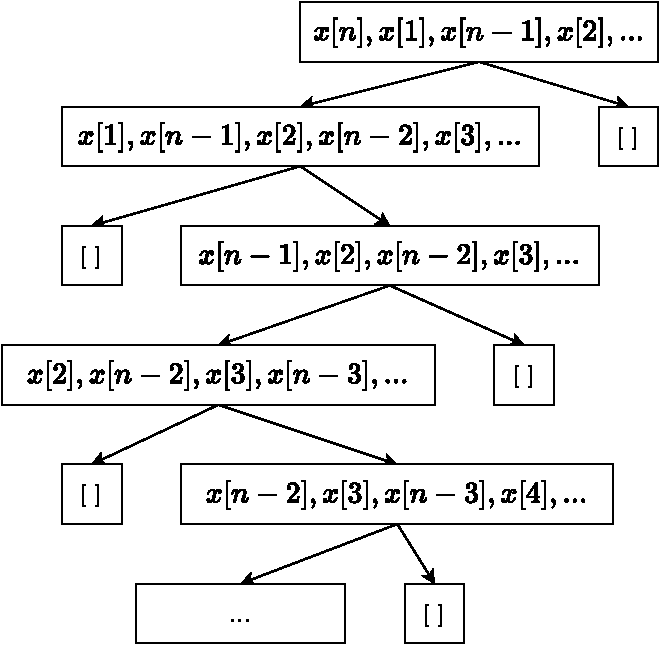
\includegraphics[scale=0.5]{img/unbalanced-zigzag}} \\
   \caption{更多最差情况}
   \label{fig:worst-cases-2}
\end{figure}

这几种最差情况中,选择第一个元素作为基准使得划分结果不平衡。塞奇维克给出了一种改进\cite{qsort-impl}:不在固定的位置上选择基准,而是进行简单的抽样以减小引发不平衡划分的可能性。检查第一个元素、中间元素、末尾元素,选择这三个元素的中数作为基准。有两种方法来寻找中数,一种最多需要三次比较操作\cite{3-way-part};另外一种通过交换将三个元素中的最小值移动到第一个元素的位置,将最大值移动到最后一个位置,将中数移动到中间。

\begin{algorithmic}[1]
\Procedure{Sort}{$A, l, u$}
  \If{$u - l > 1$}
    \State $m \gets \lfloor \dfrac{l + u}{2} \rfloor$ \Comment{或使用$l + \dfrac{u - l}{2}$避免溢出}
    \If{$A[m] < A[l]$} \Comment{确保$A[l] \leq A[m]$}
      \State \textproc{Exchange} $A[l] \leftrightarrow A[m]$
    \EndIf
    \If{$A[u-1] < A[l]$} \Comment{确保$A[l] \leq A[u-1]$}
      \State \textproc{Exchange} $A[l] \leftrightarrow A[u-1]$
    \EndIf
    \If{$A[u-1] < A[m]$} \Comment{确保$A[m] \leq A[u-1]$}
      \State \textproc{Exchange} $A[m] \leftrightarrow A[u-1]$
    \EndIf
    \State \textproc{Exchange} $A[l] \leftrightarrow A[m]$
    \State $(i, j) \gets $ \Call{Partition}{$A, l, u$}
    \State \Call{Sort}{$A, l, i$}
    \State \Call{Sort}{$A, j, u$}
  \EndIf
\EndProcedure
\end{algorithmic}

对上述四种特殊的最差情况,这一实现性能良好。它被称为“三点中值”算法。另一种常见方法是随机选择元素作为基准:

\begin{algorithmic}[1]
\Procedure{Sort}{$A, l, u$}
  \If{$u - l > 1$}
    \State \textproc{Exchange} $A[l] \leftrightarrow A[$ \Call{Random}{$l, u$} $]$
    \State $(i, j) \gets $ \Call{Partition}{$A, l, u$}
    \State \Call{Sort}{$A, l, i$}
    \State \Call{Sort}{$A, j, u$}
  \EndIf
\EndProcedure
\end{algorithmic}

函数\textproc{Random}($l, u$)返回一个在$l$和$u$之间的随机整数$l \leq i < u$。这一位置上的元素被交换到最左侧作为基准。这一方法称为\textbf{随机快速排序}\cite{CLRS}。无论是三点中值还是随机快速排序都不能完全避免最差情况。如果序列随机分布,无论选择第一个还是其它位置上的元素作为基准,在效果上都是相同的。即使在理论上无法避免最差情况,但是这些方法在实际应用中往往能够取得很好的结果。

还有一些工程实践,它们不是着眼于解决划分的最差情况。塞奇维克观察到在序列较短时,快速排序没有明显优势,而插入排序反而更快\cite{Bentley}\cite{3-way-part}。塞奇维克、本特利、麦基尔罗伊测试了不同的序列长度,定义了一个阈值。如果序列中的元素个数少于阈值,就转而使用插入排序。

\begin{algorithmic}[1]
\Procedure{Sort}{$A, l, u$}
  \If{$u - l > $ \textproc{Cut-Off}}
    \State \Call{Quick-Sort}{$A, l, u$}
  \Else
    \State \Call{Insertion-Sort}{$A, l, u$}
  \EndIf
\EndProcedure
\end{algorithmic}

\subsection{快速排序与树排序}

“真正的快速排序”复合应用了多种改进——当序列较短时转为插入排序,就地交换元素,使用三点中值选择基准,双向扫描三路划分。简短的递归定义虽然诠释了快速排序的思路,却没有使用上述任何改进。有人认这样的快速排序本质上是树排序。快速排序和树排序的确有紧密的关系。理查德$\cdot$伯德给出了如何通过“砍伐”概念\footnote{deforestation},从二叉树排序推导出快速排序\cite{algo-fp}。定义\textit{unfold}函数将一个列表转换为二叉搜索树:

\be
\begin{array}{rcl}
\textit{unfold}\ [\ ] & = & \nil \\
\textit{unfold}\ (x \cons xs) & = & (\textit{unfold}\ [a | a \in xs, a \leq x], x, \textit{unfold}\ [a | a \in xs, a > x]) \\
\end{array}
\ee

和二叉搜索树(见第二章)插入算法相比,\textit{unfold}产生树的方式大相径庭。如果列表为空,结果为一棵空树;否则,将列表中第一个元素$x$作为节点的值,然后递归地构造左右子树。其中左子树是$\leq x$的元素;而右子树是$> x$的元素。而将一棵二叉搜索树通过中序遍历转换成列表的定义为:

\be
\begin{array}{rcl}
\textit{toList}\ \nil & = & [\ ] \\
\textit{toList}\ (l, k, r) & = & \textit{toList}\ l \doubleplus [k] \doubleplus \textit{toList}\ r \\
\end{array}
\ee

我们可以将上述两个函数组合起来,定义出快速排序算法:

\be
\textit{sort} = \textit{toList} \circ \textit{unfold}
\ee

我们先通过\textit{unfold}构造出二叉搜索树,将其作为中间结果送入\textit{toList}得出列表后就可以将树丢弃了。如果将这一临时的中间结果树消除,就得到了基本的快速排序算法\cite{slpj-book-1987}。

\section{归并排序}
\index{归并排序} \index{归并排序!定义}

快速排序在大多数情况下性能优异,但在最差情况下出现退化。即使辅以各种改进也无法完全避免最差情况。归并排序在所有情形下都保证$O(n \lg n)$的复杂度,在算法设计和分析上具有重要意义。归并排序对数组和列表都适用,很多编程环境适用归并排序作为标准的排序方案\footnote{如Haskell, Python和Java}。归并排序本质上也利用了分而治之的策略。它保证划分是严格平衡的,每次将序列从中间位置分开,递归进行排序,然后将两个已序序列归并。

\be
\begin{array}{rcl}
sort\ [\ ] & = & [\ ] \\
sort\ [x] & = & [x] \\
sort\ xs & = & merge\ (sort\ as)\ (sort\ bs), \text{其中}: (as, bs) = \textit{halve}\ xs
\end{array}
\ee

其中\textit{halve}将序列对半分开。对于数组,我们可以利用索引直接在中间位置分割:$\textit{splitAt}\ \lfloor \dfrac{|xs|}{2} \rfloor\ xs$。对于列表我们需要线性时间移动到中点进行分割(见第一章),例如:

\be
\textit{splitAt}\ n\ xs = \textit{shift}\ n\ [\ ]\ xs
\ee

其中:

\be
\begin{array}{rcl}
\textit{shift}\ 0\ as\ bs & = & (as, bs) \\
\textit{shift}\ n\ as\ (b \cons bs) & = & \textit{shift}\ (n - 1)\ (b \cons as)\ bs
\end{array}
\ee

对半拆分并不需要保持顺序,我们可以利用奇偶位置分割进行简化。奇偶要么同样多,要么仅相差一个,总能保证平衡。$\textit{halve} = \textit{split}\ [\ ]\ [\ ]$,其中:

\be
\begin{array}{rcl}
\textit{split}\ as\ bs\ [\ ] & = & (as, bs) \\
\textit{split}\ as\ bs\ [x] & = & (x \cons as, bs) \\
\textit{split}\ as\ bs\ (x \cons y \cons xs) & = & \textit{split}\ (x \cons as)\ (y \cons bs)\ xs \\
\end{array}
\ee

我们也可以利用叠加操作进一步简化,如下面的例子程序,每次总把元素$x$添加到$as$上,然后交换$as \leftrightarrow bs$:

\begin{Haskell}
halve = foldr f ([], []) where
  f x (as, bs) = (bs, x : as)
\end{Haskell}

\subsection{归并}
\index{归并排序!归并}

归并的思想如图\cref{fig:merge}所示。考虑两队孩子,已分别按照身高排队。我们要求孩子们依次通过一扇门,每次一人,按照身高顺序。由于两队都已序,我们比较两个排头,个子较小的一个通过门;然后重复这一步骤,直到任何一队的孩子都已经通过,此后剩下的一队中的孩子们可以逐一通过这扇门。

\begin{figure}[htbp]
 \centering
 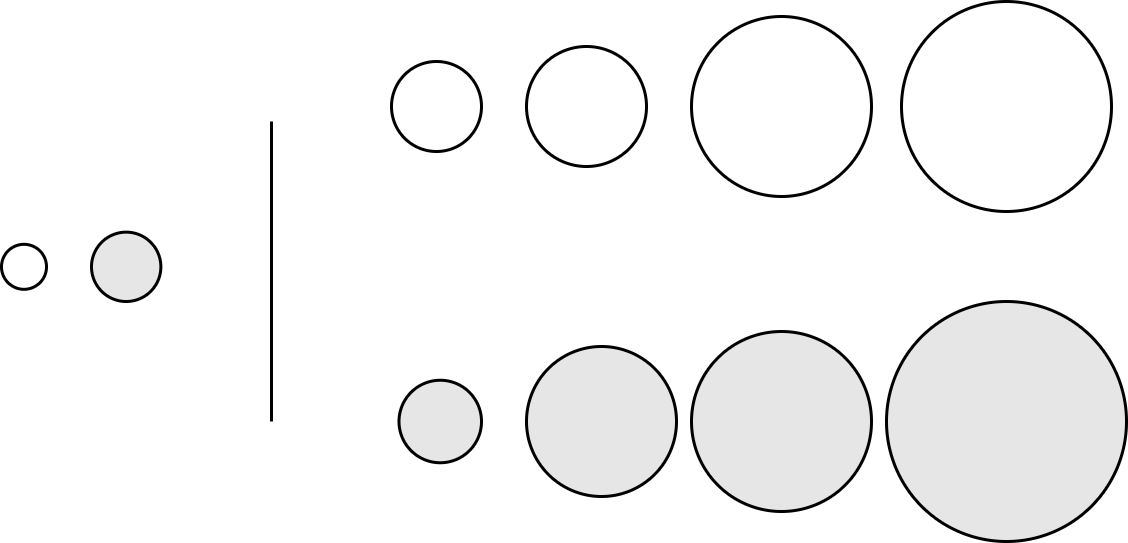
\includegraphics[scale=0.5]{img/merge2w}
 \caption{归并}
 \label{fig:merge}
\end{figure}

\be
\begin{array}{rcl}
\textit{merge}\ [\ ]\ bs & = & bs \\
\textit{merge}\ as\ [\ ] & = & as \\
\textit{merge}\ (a \cons as)\ (b \cons bs) & = & \begin{cases}
  a < b: & a : \textit{merge}\ as\ (b \cons bs) \\
  \text{否则}: & b : \textit{merge}\ (a \cons as)\ bs
  \end{cases}
\end{array}
\ee

对于数组,我们可以直接在中点位置分割,分别递归排序后归并:

\begin{algorithmic}[1]
\Procedure{Sort}{$A$}
  \State $n \gets |A|$
  \If{$n > 1$}
    \State $m \gets \lfloor \dfrac{n}{2} \rfloor$
    \State $X \gets$ \Call{Copy-Array}{$A[1...m]$}
    \State $Y \gets$ \Call{Copy-Array}{$A[m+1...n]$}
    \State \Call{Sort}{$X$}
    \State \Call{Sort}{$Y$}
    \State \Call{Merge}{$A, X, Y$}
  \EndIf
\EndProcedure
\end{algorithmic}

这一方法使用了和数组$A$同样大小的额外空间。这是由于\textproc{Merge}算法不是在原地修改元素的。归并时,我们不断检查数组$X$、$Y$中的元素,选择较小的一个放回数组$A$,接着继续向前处理直到处理完任一数组。最后把另一个数组中的剩余元素添加到$A$中。

\begin{algorithmic}[1]
\Procedure{Merge}{$A, X, Y$}
  \State $i \gets 1, j\gets 1, k\gets 1$
  \State $m \gets |X|, n \gets |Y|$
  \While{$i \leq m$ 且 $j \leq n$}
    \If{$X[i] < Y[j]$}
      \State $A[k] \gets X[i]$
      \State $i \gets i + 1$
    \Else
      \State $A[k] \gets Y[j]$
      \State $j \gets j + 1$
    \EndIf
    \State $k \gets k + 1$
  \EndWhile
  \While{$i \leq m$}
    \State $A[k] \gets X[i]$
    \State $k \gets k + 1$
    \State $i \gets i + 1$
  \EndWhile
  \While{$j \leq n$}
    \State $A[k] \gets Y[j]$
    \State $k \gets k + 1$
    \State $j \gets j + 1$
  \EndWhile
\EndProcedure
\end{algorithmic}

\subsection{性能分析}
\index{归并排序!性能分析}

归并排序分为两步:划分和归并。我们总把序列对半分割。划分树是一棵平衡的二叉树,如图\cref{fig:qsort-best}所示。树的高度为$O(\lg n)$。归并排序的递归深度为$O(\lg n)$。在每一层都进行归并。归并逐一比较两个序列的元素,当其中一个处理完,将另一序列中的剩余元素复制到结果中。归并的复杂度为线性时间。如果序列长度为$n$,记$T(n)$为排序所时间,我们有一下递归关系:

\be
T(n) = T(\dfrac{n}{2}) + T(\dfrac{n}{2}) + c n = 2 T(\dfrac{n}{2}) + c n
\ee

排序时间包含三部分:对前半部分排序$T(\dfrac{n}{2})$,对后半部分排序$T(\dfrac{n}{2})$,归并$c n$,其中$c$是某个常数。解此方程得到结果为$O(n \lg n)$。另外一个重要性能指标是空间复杂度。不同的归并方法空间消耗大相径庭。我们稍后针对几种实现给出空间复杂度分析。对上面的基本实现,每次递归时,都需要和输入数组同样大小的空间,用以复制元素和进一步的递归。递归返回后,这些空间可以释放。最大的空间消耗出现在进入最深一层递归时,为$O(n \lg n)$。

\subsection{改进}
\index{归并排序!分配工作区}

为了简化归并$X$、$Y$逻辑,我们将$\infty$添加到它们末尾\footnote{降序使用$-\infty$}。

\begin{algorithmic}[1]
\Procedure{Merge}{$A, X, Y$}
  \State \Call{Append}{$X, \infty$}
  \State \Call{Append}{$Y, \infty$}
  \State $i \gets 1, j\gets 1, n \gets |A|$
  \For{$k \gets$ from 1 to $n$}
    \If{$X[i] < Y[j]$}
      \State $A[k] \gets X[i]$
      \State $i \gets i + 1$
    \Else
      \State $A[k] \gets Y[j]$
      \State $j \gets j + 1$
    \EndIf
  \EndFor
\EndProcedure
\end{algorithmic}

在归并时反复获取空间复制数组是一个瓶颈\cite{Bentley}。我们可以一次性准备好和数组$A$同样大小的工作区。递归时复用这个工作区进行归并。最后再把工作区的内容复制回原数组。

\begin{algorithmic}[1]
\Procedure{Sort}{A}
  \State $n \gets |A|$
  \State \textproc{Sort$'$}$(A$, \Call{Create-Array}{$n$}, $1, n)$
\EndProcedure
\Statex
\Procedure{Sort$'$}{$A, B, l, u$}
  \If{$u - l > 0$}
    \State $m \gets \lfloor \dfrac{l + u}{2} \rfloor$
    \State \Call{Sort$'$}{$A, B, l, m$}
    \State \Call{Sort$'$}{$A, B, m + 1, u$}
    \State \Call{Merge$'$}{$A, B, l, m, u$}
  \EndIf
\EndProcedure
\end{algorithmic}

我们同时需要修改\textproc{Merge$'$}使用传入的工作区:

\begin{algorithmic}[1]
\Procedure{Merge$'$}{$A, B, l, m, u$}
  \State $i \gets l, j \gets m + 1, k \gets l$
  \While{$i \leq m$ 且 $j \leq u$}
    \If{$A[i] < A[j]$}
      \State $B[k] \gets A[i]$
      \State $i \gets i + 1$
    \Else
      \State $B[k] \gets A[j]$
      \State $j \gets j + 1$
    \EndIf
    \State $k \gets k + 1$
  \EndWhile
  \While{$i \leq m$}
    \State $B[k] \gets A[i]$
    \State $k \gets k + 1$
    \State $i \gets i + 1$
  \EndWhile
  \While{$j \leq u$}
    \State $B[k] \gets A[j]$
    \State $k \gets k + 1$
    \State $j \gets j + 1$
  \EndWhile
  \For{$i \gets$ from $l$ to $u$} \Comment{复制回}
    \State $A[i] \gets B[i]$
  \EndFor
\EndProcedure
\end{algorithmic}

这一改进降空间复杂度从$O(n \lg n)$降低到$O(n)$。对于10万个整数元素排序,性能可提升20\%到25\%。

\subsection{原地归并排序}
\index{归并排序!原地归并排序}

为了避免使用额外的空间,我们考虑如何复用原数组作为工作区。如图\cref{fig:merge-in-place-naive}所示,子数组$X$和$Y$已排序好,当进行原地归并时,令$l$之前为已归并部分,所有元素已序。若$A[l] < A[m]$,就向前移动$l$一步;否则若$A[l] \geq A[m]$需要把$A[m]$放入归并结果中,位于$l$之前。为此,我们把所有$l$和$m$之间的元素(包括$l$)向后平移一个位置。

\begin{figure}[htbp]
 \centering
      \begin{tikzpicture}[scale=0.8]
      \draw (0, 0) rectangle (3, 1) node [pos=.5] {已归并}
            (3, 0) rectangle (4, 1) node [pos=.5] {$A[l]$}
            (4, 0) rectangle (8, 1) node (subA) [pos=.5] {...已序部分$X$...}
            (8, 0) rectangle (9, 1) node (xsj) [pos=.5] {$A[m]$}
            (9, 0) rectangle (13, 1) node [pos=.5] {...已序部分$Y$...};
      \draw[thick, ->] (subA) edge [bend right=45] node [below] {若$A[l] \geq A[m]$则平移$X$} (xsj);
      \end{tikzpicture}
 \caption{原地平移归并}
 \label{fig:merge-in-place-naive}
\end{figure}

\begin{algorithmic}[1]
\Procedure{Merge}{$A, l, m, u$}
  \While{$l \leq m \leq u$}
    \If{$A[l] < A[m]$}
      \State $l \gets l + 1$
    \Else
      \State $x \gets A[m]$
      \For{$i \gets m $ down-to $l+1$} \Comment{平移}
        \State $A[i] \gets A[i-1]$
      \EndFor
      \State $A[l] \gets x$
    \EndIf
  \EndWhile
\EndProcedure
\end{algorithmic}

\index{归并排序!原地工作区}
但这一原地平移的时间复杂度退化成$O(n^2)$。数组的移动是一个线性时间的操作,它和$X$中的元素个数成正比。当对子数组排序时,我们使用数组剩余的部分作为工作区。对那些已在工作区内的元素,要避免它们被覆盖丢失。当比较已序子数组$A$和$B$的元素时,每当把较小的元素放入工作区中的某个位置时,我们同时将工作区中的元素交换出来。归并完成后,原来的两个子数组就保存了此前工作区的内容。如图\cref{fig:merge-workarea}所示。

\begin{figure}[htbp]
 \centering
      \begin{tikzpicture}[scale=0.8]
      \draw (0, 2) rectangle (3, 3) node [pos=.5] {...复用...}
            (3, 2) rectangle (4, 3) node (ai) [pos=.5] {$A[i]$}
            (4, 2) rectangle (5, 3) node [pos=.5] {...}
            (7, 2) rectangle (10, 3) node [pos=.5] {...复用...}
            (10, 2) rectangle (11, 3) node (bj) [pos=.5] {$B[j]$}
            (11, 2) rectangle (12, 3) node [pos=.5] {...}
            (0, 0) rectangle (3, 1) node [pos=.5] {...已归并...}
            (3, 0) rectangle (4, 1) node (ck) [pos=.5] {$C[k]$}
            (4, 0) rectangle (5, 1) node [pos=.5] {...};
      \draw[thick, <->] (ai) edge [bend left] node [above] {比较} (bj)
                        (ai) edge node [right] {若$A[i] < B[j]$,则交换$A[i] \leftrightarrow C[k]$} (ck);
      \end{tikzpicture}
 \caption{归并时将工作区内容交换出来}
 \label{fig:merge-workarea}
\end{figure}

已序子数组$A$、$B$和工作区$C$都是原数组的一部分。归并时需要提供的参数包括:$A$、$B$的起始、结束位置,分别用区间$[i, m)$、$[j, n)$表示\footnote{$[a, b)$表示左闭右开区间,包括$a$,但不包括$b$。};工作区的起始位置$k$。

\begin{algorithmic}[1]
\Procedure{Merge}{$A, [i, m), [j, n), k$}
  \While{$i < m$ 且 $j < n$}
    \If{$A[i] < A[j]$}
      \State \textproc{Exchange} $A[k] \leftrightarrow A[i]$
      \State $i \gets i + 1$
    \Else
      \State \textproc{Exchange} $A[k] \leftrightarrow A[j]$
      \State $j \gets j + 1$
    \EndIf
    \State $k \gets k + 1$
  \EndWhile
  \While{$i < m$}
    \State \textproc{Exchange} $A[k] \leftrightarrow A[i]$
    \State $i \gets i + 1$
    \State $k \gets k + 1$
  \EndWhile
  \While{$j < m$}
    \State \textproc{Exchange} $A[k] \leftrightarrow A[j]$
    \State $j \gets j + 1$
    \State $k \gets k + 1$
  \EndWhile
\EndProcedure
\end{algorithmic}

归并工作区需要满足两个条件:

\begin{enumerate}
\item 工作区必须足够大,以容纳交换进来的元素而不越界;
\item 工作区可以和任一子数组重叠,但须保证不会覆盖尚未归并的元素。
\end{enumerate}

我们可以用一半数组作为工作区,将另一半归并排序。如图\cref{fig:merge-in-place-start}所示。

\begin{figure}[htbp]
 \centering
      \begin{tikzpicture}[scale=0.8]
      \draw (0, 0) rectangle (3, 1) node [pos=.5] {...未排序...}
            (3, 0) rectangle (6, 1) node [pos=.5] {...已排序...};
      \end{tikzpicture} \\
 \caption{归并排序一半数组}
 \label{fig:merge-in-place-start}
\end{figure}

如果再递归地对一半工作区排序,就只剩下$\dfrac{1}{4}$尚未排序了。如图\cref{fig:merge-in-place-quater}所示。我们必须在某个时刻归并$A$($\dfrac{1}{2}$数组)和$B$($\dfrac{1}{4}$数组)。但剩余工作区大小只能容纳$\dfrac{1}{4}$数组,不能容纳$A + B$的结果。

\begin{figure}[htbp]
 \centering
 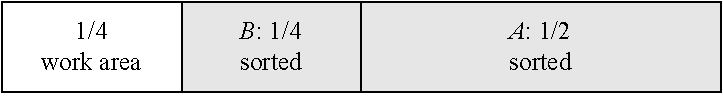
\includegraphics[scale=0.8]{img/workarea-1}
 \caption{需要在某个时刻归并$A$、$B$}
 \label{fig:merge-in-place-quater}
\end{figure}

工作区的第二条规则启发我们:通过某种设计,使得未归并的元素不被覆盖,从而利用工作区和子数组的重叠部分来解决问题。我们先对工作区的后1/2排序,结果$B$被交换到前1/2部分,新工作区就位于$A$、$B$中间,如图\cref{fig:merge-in-place-setup}上方所示。这样的安排使得工作区和子数组$A$产生了重叠\cite{msort-in-place}。考虑两种极端情况:

\begin{figure}[htbp]
 \centering
 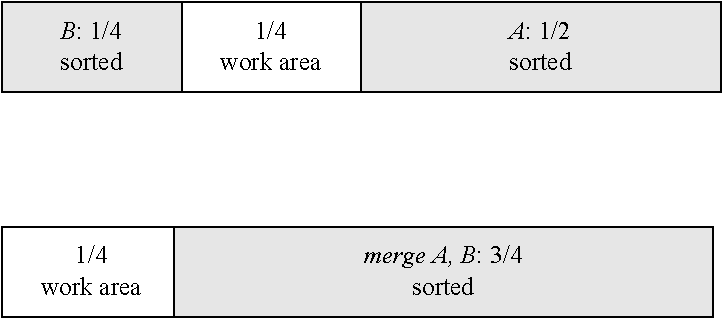
\includegraphics[scale=0.8]{img/workarea-2}
 \caption{利用工作区归并$A$、$B$}
 \label{fig:merge-in-place-setup}
\end{figure}

\begin{enumerate}
\item 所有$B$中元素都小于$A$中任意元素。归并后,$B$中全部内容移动到工作区中,而$B$中包括以前工作区中的内容。由于工作区和$B$的大小相等,因此恰好可以交换它们;
\item 所有$A$中元素都小于$B$中任意元素。归并不断交换$A$和工作区中的内容。当工作区被$A$中一半元素填满后,开始覆盖$A$中的内容。幸运的是,被覆盖的是已归并的元素。工作区的右侧边界不断向数组的末尾移动到3/4的位置。此后,归并算法开始交换$B$和工作区的内容。最终工作区被移动到了数组最左侧,如图\cref{fig:merge-in-place-setup}下方所示。
\end{enumerate}

其它情况介于两种极端情况之间,最终工作区被移动到前1/4。我们重复这一步骤,总是对未排序部分的后1/2排序,将结果交换到前1/2,而使新工作区位于中间。不断将工作区的大小减半,从$\dfrac{1}{2}$到$\dfrac{1}{4}$到$\dfrac{1}{8}$……归并的规模不断下降。当工作区中只剩下一个元素时结束。归并只有一个元素的数组等价于插入。我们可以使用插入排序来处理最后的几个元素。

\begin{algorithmic}[1]
\Procedure{Sort}{$A, l, u$}
  \If{$u - l > 0$}
    \State $m \gets \lfloor \dfrac{l + u}{2} \rfloor$
    \State $w \gets l + u - m$
    \State \Call{Sort'}{$A, l, m, w$} \Comment{对一半数组排序}
    \While{$w - l > 1$}
      \State $u' \gets w$
      \State $w \gets \lceil \dfrac{l + u'}{2} \rceil$ \Comment{工作区减半}
      \State \Call{Sort'}{$A, w, u', l$} \Comment{对剩余一半排序}
      \State \Call{Merge}{$A, [l, l + u' - w), [u', u), w$}
    \EndWhile
    \For{$i \gets w$ down-to $l$} \Comment{改用插入排序}
      \State $j \gets i$
      \While{$j \leq u$ 且 $A[j] < A[j-1]$}
        \State \textproc{Exchange} $A[j] \leftrightarrow A[j-1]$
        \State $j \gets j + 1$
      \EndWhile
    \EndFor
  \EndIf
\EndProcedure
\end{algorithmic}

为了保证工作区足够大,我们使用上限取整。我们将包含结束位置的区间信息传入了\textproc{Merge}算法。接下来,我们需要定义\textproc{Sort'}算法,它反过来递归调用\textproc{Sort}来交换工作区和已序部分。

\begin{algorithmic}[1]
\Procedure{Sort'}{$A, l, u, w$}
  \If{$u - l > 0$}
    \State $m \gets \lfloor \dfrac{l + u}{2} \rfloor$
    \State \Call{Sort}{$A, l, m$}
    \State \Call{Sort}{$A, m+1, u$}
    \State \Call{Merge}{$A, [l, m), [m+1, u), w$}
  \Else \Comment{将所有元素交换到工作区}
    \While{$l \leq u$}
      \State \textproc{Exchange} $A[l] \leftrightarrow A[w]$
      \State $l \gets l + 1$
      \State $w \gets w + 1$
    \EndWhile
  \EndIf
\EndProcedure
\end{algorithmic}

这一方法在归并中并不平移子数组。未排序部分不断递减:$\dfrac{n}{2}, \dfrac{n}{4}, \dfrac{n}{8}, ...$,总共需要$O(\lg n)$步完成排序。每次递归对剩余部分的一半排序,然后使用线性时间进行归并。令$n$个元素排序时间为$T(n)$,我们有如下递归关系:

\be
T(n) = T(\frac{n}{2}) + c \frac{n}{2} + T(\frac{n}{4}) + c \frac{3n}{4} + T(\frac{n}{8}) + c \frac{7n}{8} + ...
\label{eq:in-place-sort-time}
\ee

对于一半的元素,花费的时间为:

\be
T(\frac{n}{2}) = T(\frac{n}{4}) + c \frac{n}{4} + T(\frac{n}{8}) + c \frac{3n}{8} + T(\frac{n}{16}) + c \frac{7n}{16} + ...
\label{eq:in-place-sort-time-half}
\ee

两式相减(\cref{eq:in-place-sort-time}) - (\cref{eq:in-place-sort-time-half})得:

\[
T(n) - T(\frac{n}{2}) = T(\frac{n}{2}) + c n (\frac{1}{2} + \frac{1}{2} + ... )
\]

共有$\lg n$个$\dfrac{1}{2}$相加,由此得到计算时间的递归关系为:

\[
T(n) = 2 T(\frac{1}{2}) + \frac{c}{2} n \lg n
\]

使用裂项求和法解方程,得到结果$O(n \lg^2 n)$。

\subsection{自然归并排序}
\index{归并排序!自然归并排序}

\begin{figure}[htbp]
 \centering
 \includegraphics[scale=0.25]{img/burn-candle-2-ends}
 \caption{从两端向中间燃烧的蜡烛}
 \label{fig:burn-candle}
\end{figure}

高德纳给出了另外一种方法来实现分而治之的归并排序。整个过程如同从两端点燃一支蜡烛\cite{TAOCP},称为自然归并排序算法。对于任何序列,可以在任何位置开始找到一个非递减子序列。作为一个特殊情况,我们总可以在最左侧找到这样的子序列。下表给出了一些例子,非递减子序列用下划线标出。

\btab{l}
\underline{15}, 0, 4, 3, 5, 2, 7, 1, 12, 14, 13, 8, 9, 6, 10, 11 \\
\underline{8, 12, 14}, 0, 1, 4, 11, 2, 3, 5, 9, 13, 10, 6, 15, 7 \\
\underline{0, 1, 2, 3, 4, 5, 6, 7, 8, 9, 10, 11, 12, 13, 14, 15} \\
\etab

表中的第一行描述了最短情况,第二个元素小于第一个,因此非递减子序列长度为一,只包含第一个元素;表中的最后一行描述了最长情况,整个序列已序,非递减子序列包含全部元素。对称地,我们总是可以从右向左找到一个非递减子序列。于是,我们可以将两个非递减子序列,一个从头部开始,一个从尾部开始,归并成一个更长的序列。这一思路的特点是,我们可以利用元素间的自然顺序进行划分。

\begin{figure}[htbp]
 \centering
 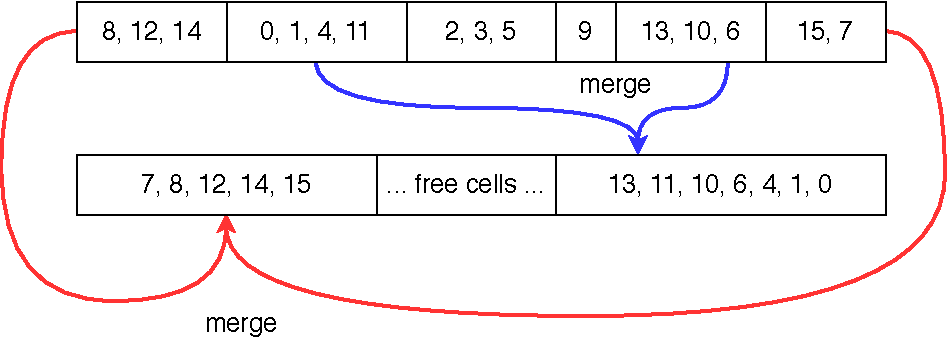
\includegraphics[scale=0.8]{img/nature-merge-sort}
 \caption{自然归并排序}
 \label{fig:nature-merge-sort}
\end{figure}

图\cref{fig:nature-merge-sort}描述了这一思路。算法开始时,我们从两侧扫描序列,分别找到最长的非递减子序列。然后这两个子序列被归并到一个工作区的左侧。接着,我们重复这一步骤,继续从两侧向中心进行扫描。这一次,我们将两个子序列归并到工作区的右侧,从右向左放置。这样左右交替向工作区中心推进。当所有元素都被扫描归并到工作区后,我们交换工作区和原数组,再次从两侧向中心扫描归并。开始新一轮的扫描时,如果发现最长的非递减子序列一直伸展到末尾,说明整个序列已序,排序结束。这一方法从左右两个方向处理数组,并且使用子序列的自然顺序,它被称为\textbf{两路自然归并}排序。如图\cref{fig:nature-msort-invariant}所示,任何时候,$a$之前$d$之后的元素已处理完。我们将非递减子序列$[a, b)$向右扩展到最长,同时将子序列$[c, d)$向左扩展到最长。对于工作区,$f$之前和$r$之后的元素都已归并好(包含若干子序列)。奇数轮时,我们将子序列$[a, b)$和$[c, d)$从$f$起向右归并;偶数轮时,我们将子序列从$r$起向左归并。

\captionsetup[subfigure]{labelformat=empty, margin=10pt}
\begin{figure}[htbp]
 \centering
   \subcaptionbox{}{
      \begin{tikzpicture}[scale=0.8]
      \draw (0, 0) rectangle (3, 1) node [pos=.5] {...已扫描...}
            (3, 0) rectangle (6, 1) node [pos=.5] {...扩展$[a, b)$...}
            (6, 0) rectangle (8, 1) node [pos=.5] {...?...}
            (8, 0) rectangle (11, 1) node [pos=.5] {...扩展$[c, d)$...}
            (11, 0) rectangle (14, 1) node [pos=.5] {...已扫描...};
      \fill [black] (3, 0) rectangle (3.1, 1) node (abar) [pos=.5] {}
                    (6, 0) rectangle (6.1, 1) node (bbar) [pos=.5] {}
                    (8, 0) rectangle (8.1, 1) node (cbar) [pos=.5] {}
                    (11, 0) rectangle (11.1, 1) node (dbar) [pos=.5] {};
      \draw (3, 2) node (a) {a}
            (6, 2) node (b) {b}
            (8, 2) node (c) {c}
            (11, 2) node (d) {d};
      \draw[thick, ->] (a) edge [bend right] (abar)
                       (b) edge [bend right] (bbar)
                       (c) edge [bend left] (cbar)
                       (d) edge [bend left] (dbar);
      \end{tikzpicture}} \\
    \subcaptionbox{}{
      \begin{tikzpicture}[scale=0.8]
      \draw (0, 0) rectangle (3, 1) node [pos=.5] {...已归并...}
            (3, 0) rectangle (8, 1) node [pos=.5] {...未使用...}
            (8, 0) rectangle (11, 1) node [pos=.5] {...已归并...};
      \fill [black] (3, 0) rectangle (3.1, 1) node (fbar) [pos=.5] {}
                    (8, 0) rectangle (8.1, 1) node (rbar) [pos=.5] {};
      \draw (3, 2) node (f) {f}
            (8, 2) node (r) {r};
      \draw[thick, ->] (f) edge [bend right] (fbar)
                       (r) edge [bend right] (rbar);
      \end{tikzpicture}} \\
 \caption{自然归并排序时的不变性质}
 \label{fig:nature-msort-invariant}
\end{figure}
\captionsetup[subfigure]{labelformat=parens}

在排序开始前,我们准备好和数组同样大小的工作区。$a$和$b$指向最左侧,$c$和$d$指向最右侧。$f$、$r$指向工作区左右两端。

\begin{algorithmic}[1]
\Function{Sort}{$A$}
  \If{$|A| > 1$}
    \State $n \gets |A|$
    \State $B \gets$ \Call{Create-Array}{$n$}  \Comment{创建工作区}
    \Loop
      \State $[a, b) \gets [1, 1)$
      \State $[c, d) \gets [n+1, n+1)$
      \State $f \gets 1, r \gets n$ \Comment{指向工作区首尾}
      \State $t \gets 1$            \Comment{奇偶轮}
      \While{$b < c$}               \Comment{存在需要扫描的元素}
        \Repeat \Comment{扩展$[a, b)$}
          \State $b \gets b + 1$
        \Until{$b \geq c$ 或 $A[b] < A[b-1]$}

        \Repeat \Comment{扩展$[c, d)$}
          \State $c \gets c - 1$
        \Until{$c \leq b$ 或 $A[c-1] < A[c]$}

        \If{$c < b$} \Comment{避免交错}
          \State $c \gets b$
        \EndIf

        \If{$b - a \geq n$} \Comment{$[a, b)$覆盖全数组时排序结束}
          \State \Return $A$
        \EndIf

        \If{$t$是奇数} \Comment{从左归并}
          \State $f \gets$ \Call{Merge}{$A, [a, b), [c, d), B, f, 1$}
        \Else \Comment{从右归并}
          \State $r \gets$ \Call{Merge}{$A, [a, b), [c, d), B, r, -1$}
        \EndIf
        \State $a \gets b, d \gets c$
        \State $t \gets t + 1$
      \EndWhile
      \State \textproc{Exchange} $A \leftrightarrow B$ \Comment{切换工作区}
    \EndLoop
  \EndIf
  \State \Return $A$
\EndFunction
\end{algorithmic}

归并时需要将归并方向作为参数传入。

\begin{algorithmic}[1]
\Function{Merge}{$A, [a, b), [c, d), B, w, \Delta$}
  \While{$a < b$ 且 $c < d$}
    \If{$A[a] < A[d-1]$}
      \State $B[w] \gets A[a]$
      \State $a \gets a + 1$
    \Else
      \State $B[w] \gets A[d-1]$
      \State $d \gets d - 1$
    \EndIf
    \State $w \gets w + \Delta$
  \EndWhile
  \While{$a < b$}
    \State $B[w] \gets A[a]$
    \State $a \gets a + 1$
    \State $w \gets w + \Delta$
  \EndWhile
  \While{$c < d$}
    \State $B[w] \gets A[d-1]$
    \State $d \gets d - 1$
    \State $w \gets w + \Delta$
  \EndWhile
  \State \Return $w$
\EndFunction
\end{algorithmic}

自然归并排序的性能看似和数组中元素顺序相关。假设运气不佳,第一轮扫描时,非递减子序列的长度总为1。这轮结束后,工作区中归并的已序子数组的长度为2。假设接下来一轮运气仍然很差,但是现在非递减子序列的长度已不可能小于2。这一轮后,工作区包含长度至少为4的归并结果……每一轮后,归并的已序子数组的长度都加倍,因此最多需要$O(\lg n)$轮扫描归并。每一轮扫描所有的元素,所以总性能为$O(n \lg n)$。如果元素存储在列表中,我们无法从首尾两端扫描。考虑列表由若干非递减子列表组成,我们可以每次取两个子列表归并。反复取出归并后,非递减子列表的数目不断减半,最后得到排序结果。这个过程可定义如下(柯里化):

\be
sort = sort' \circ group
\ee

其中$group$将元素分组为非递减子列表:

\be
\begin{array}{rcl}
\textit{group}\ [\ ] & = & [[\ ]] \\
\textit{group}\ [x] & = & [[x]] \\
\textit{group}\ (x \cons y \cons xs) & = & \begin{cases}
  x < y: & (x \cons g) \cons gs, \text{其中}: (g \cons gs) = \textit{group}\ (y \cons xs) \\
  \text{否则}: & [x] \cons g \cons gs \\
\end{cases}
\end{array}
\ee

$sort'$把分组中子列表成对归并,然后再次结对归并直到完成排序:

\be
\begin{array}{rcl}
\textit{sort}'\ [\ ] & = & [\ ] \\
\textit{sort}'\ [g] & = & g \\
\textit{sort}'\ gs & = & \textit{sort}'\ (\textit{mergePairs}\ gs) \\
\end{array}
\ee

其中\textit{mergePairs}定义为:

\be
\begin{array}{rcl}
\textit{mergePairs}\ (g_1 \cons g_2 \cons gs) & = & merge\ g_1\ g_2 : \textit{mergePairs}\ gs \\
\textit{mergePairs}\ gs & = & gs
\end{array}
\ee

另外我们也可以用叠加操作实现$sort'$:

\be
\textit{sort}' = foldr\ merge\ [\ ]
\ee

\begin{Exercise}\label{ex:multi-merge}
\Question{使用叠加和$mergePairs$的实现复杂度相同么?如果相同,请给出证明;如果不同,哪个更快?}
\end{Exercise}

\begin{Answer}[ref = {ex:multi-merge}]
\Question{使用叠加和$mergePairs$的实现复杂度相同么?如果相同,请给出证明;如果不同,哪个更快?

这个问题本质上是合并$k$个已序序列。简化问题,设每个序列的平均长度为$n$。使用叠加相当于先合并$s_1$和空序列,$merge([\ ], s_1) = [\ ] \oplus s_1$,然后合并$s_2$,$[\ ] \oplus s_1 \oplus s_2$,然后再合并$s_3$,$[\ ] \oplus s_1 \oplus s_2 \oplus s_3$……所以总复杂度为:$O(n + 2n + 3n + 4n + ... + kn) = O(n\dfrac{k(k+1)}{2}) = O(nk^2)$。而两两合并,第一轮是$s_1 \oplus s_2$,$s_3 \oplus s_4$……用时$O(kn)$,接下来一轮:$(s_1 \oplus s_2) \oplus (s_3 \oplus s_4)$……又是$O(kn)$。总共进行$lg k$轮,总复杂度为:$O(nk \lg k)$。故两两合并的速度更快。

我们也可以利用一个大小为$k$的小顶堆,保存$k$个序列各自的最小元素进行合并,复杂度也是$O(nk \lg k)$。
}
\end{Answer}

\subsection{自底向上归并排序}
\index{归并排序!自底向上归并排序}

自然归并排序的复杂度分析给出了一种自底向上的排序方法,可以很方便地用迭代实现。首先将序列变成$n$个列表,每个列表包含一个元素。然后将相邻的子序列两两归并,得到$\frac{n}{2}$个长度为2的已序列表;如果$n$是奇数,会剩余一个长度为1的子序列。我们不断成对归并相邻子序列,最后得到排序的结果。高德纳称之为“直接两路归并排序”\cite{TAOCP},如图\cref{fig:bottom-up-msort}所示。

\begin{figure}[htbp]
 \centering
 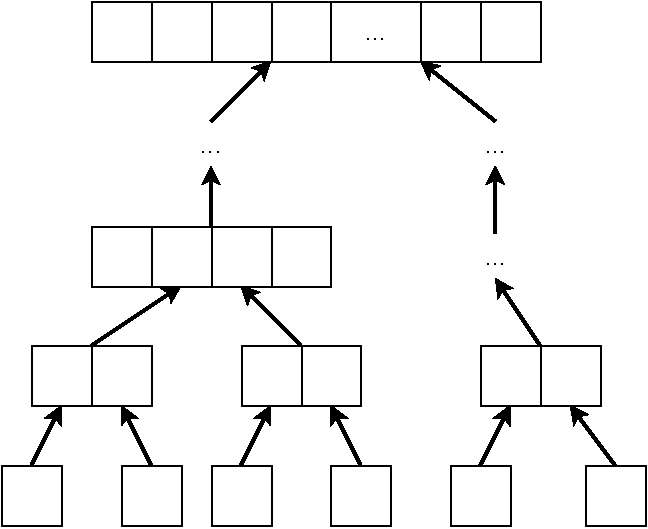
\includegraphics[scale=0.6]{img/bottom-up-msort}
 \caption{自底向上归并排序}
 \label{fig:bottom-up-msort}
\end{figure}

我们无需在每次递归时分割列表。列表$[x_1, x_2, ..., x_n]$在一开始时被分为$n$个单一元素子列表$[[x_1], [x_2], ..., [x_n]]$,然后我们不断对它们归并。

\be
sort = sort' \circ map (x \mapsto [x])
\ee

我们复用自然归并排序中的$sort'$和\textit{mergePairs}。不断成对归并子列表,直到最后一个\cite{okasaki-book}。自底向上归并排序和自然归并排序很像,仅仅是分组方法不同。本质上,它可以由自然归并排序的特殊情况(最差情况)推导出来。自然归并排序总是将非递减子列表扩展到最长,而自底向上归并排序仅把子列表的长度扩展到1。自底向上归并排序的定义是尾递归形式。我们可以消除递归转换成迭代实现:

\begin{algorithmic}[1]
\Function{Sort}{$A$}
  \State $n \gets |A|$
  \State $B \gets $ \Call{Create-Array}{$n$}
  \For{$i$ from 1 to $n$}
    \State $B[i] = [A[i]]$
  \EndFor
  \While{$n > 1$}
    \For{$i \gets $ from $1$ to $\lfloor \dfrac{n}{2} \rfloor$}
      \State $B[i] \gets$ \Call{Merge}{$B[2i -1], B[2i]$}
    \EndFor
    \If{\Call{Odd}{$n$}}
      \State $B[\lceil \dfrac{n}{2} \rceil] \gets B[n]$
    \EndIf
    \State $n \gets \lceil \dfrac{n}{2} \rceil$
  \EndWhile
  \If{$B = [\ ]$}
    \State \Return $[\ ]$
  \EndIf
  \State \Return $B[1]$
\EndFunction
\end{algorithmic}

\begin{Exercise}
\Question{使用叠加实现自底向上归并排序。}
\end{Exercise}

\section{并行处理}
\index{并行归并排序}\index{并行快速排序}

在基本快速排序算法中,当划分完成时,可以并行对两个子序列排序。这一策略对归并排序也适用。实际上,并行快速排序和归并排序,并非只有两个并行任务,而是将序列分割成$p$个子序列,其中$p$为处理器个数。理想情况下,如果我们可以并行在$T'$时间内完成排序,并且满足$O(n \lg n) = p T'$,就称为\textbf{线性加速},这样的算法叫做最优化并行算法。但是,简单地扩展基本快速排序算法:选取$p-1$个基准,划分为$p$个子序列,然后并行对它们排序,并不是最优化的。瓶颈出现在划分阶段,我们只能得到平均$O(n)$的性能。另一方面,并发归并排序算法的瓶颈出现在归并阶段。为了达到最优化的并行加速,需要对并行归并排序和快速排序进行更好的设计。总体上说,归并排序和快速排序的分治特性使它们相对容易并行化。理查德$cdot$科尔在1986年发现了使用$n$个处理器,性能为$O(\lg n)$的并行归并排序算法\cite{para-msort}。并行处理是一个巨大而复杂的题目,超出了本书“基本算法”的范围。读者可以参考\cite{para-msort}和\cite{para-qsort}了解更多内容。

\section{小结}

本章介绍了两种常用的分治排序算法:快速排序和归并排序。它们都达到了基于比较的排序算法性能上限$O(n \lg n)$。塞奇维克说快速排序是20世纪发现的最伟大的算法。大量的编程环境都使用快速排序作为标准排序工具。某些环境中,特别是在处理动态抽象序列的情况下,存储模型不是简单的数组,人们往往使用归并排序\footnote{实际中,大部分排序工具都是某种混合算法,在序列较短时使用插入排序来保持良好的性能}。这一现象的原因,可以部分地在本章中找到。快速排序在大多数情况下表现优异。和其它算法相比,快速排序需要较少的交换操作。但在另一些环境中,交换并不是最有效的操作。这是因为底层的数据结构比较复杂,不是向量化的数组。而归并排序则适合这类环境,在各种情况下都能保证性能。反之快速排序的性能在最差情况下出现退化。在命令式环境中对数组排序时,归并排序的性能不如快速排序,并且需要额外的空间进行归并。但在某些情况下,例如嵌入式系统,空间往往受到限制。原地归并排序仍然是一个活跃的研究领域。

快速排序和归并排序存在着联系。快速排序可以被看作树排序的一种优化形式。同样归并排序也可以由树排序推导出来\cite{sort-deriving}。排序算法有多种分类\cite{TAOCP}其中一种是根据划分和归并的难易程度分类\cite{algo-fp}。例如快速排序,它易于归并。因为基准前的子序列都小于等于基准后的子序列。快速排序的归并实际上就是序列的连接。与此相反,归并排序的归并过程复杂,但划分却很简单。无论是等分、奇偶分割、自然分割、还是自底向上分割。快速排序很难保证完美分割,无法完全避免最差情况。尽管人们设计另一些改进方法如三点中值法、随机快速排序、三路划分等。

到本章为止,我们给出了基本排序算法,包括插入排序、树排序、选择排序、堆排序、快速排序、归并排序。排序仍然是计算机科学中活跃的研究领域。在写这一章的时候,人们正经历着当时所谓“大数据”的挑战,传统的排序方法无法在有限的时间和资源下处理越来越巨大的数据。在某些领域,处理几百G的数据已经成为了日常工作中的任务。

\begin{Exercise}
\Question{使用归并排序的策略,设计一种算法可以从一个序列产生一棵二叉搜索树。}
\end{Exercise}

\section{附录:例子程序}

原地划分:

\begin{lstlisting}[language = Bourbaki]
Int partition([K] xs, Int l, Int u) {
    for (Int pivot = l, Int r = l + 1; r < u; r = r + 1) {
        if xs[pivot] >= xs[r] {
            l = l + 1
            swap(xs[l], xs[r])
        }
    }
    swap(xs[pivot], xs[l])
    return l + 1
}

void sort([K] xs, Int l, Int u) {
    if l < u {
        Int m = partition(xs, l, u)
        sort(xs, l, m - 1)
        sort(xs, m, u)
    }
}
\end{lstlisting}

双向扫描:

\begin{lstlisting}[language = Bourbaki]
void sort([K] xs, Int l, Int u) {
    if l < u - 1 {
        Int pivot = l, Int i = l, Int j = u
        loop {
            while i < u and xs[i] < xs[pivot] {
                i = i + 1
            }
            while j >=l and xs[pivot] < xs[j] {
                j = j - 1
            }
            if j < i then break
            swap(xs[i], xs[j])
        }
        swap(xs[pivot], xs[j])
        sort(xs, l, j)
        sort(xs, i, u)
    }
}
\end{lstlisting}

归并排序:

\begin{lstlisting}[language = Bourbaki]
[K] sort([K] xs) {
    Int n = length(xs)
    if n > 1 {
        var ys = sort(xs[0 ... n/2 - 1])
        var zs = sort(xs[n/2 ...])
        xs = merge(xs, ys, zs)
    }
    return xs
}

[K] merge([K] xs, [K] ys, [K] zs) {
    Int i = 0
    while ys != [] and zs != [] {
        xs[i] = if ys[0] < zs[0] then pop(ys) else pop(zs)
        i = i + 1
    }
    xs[i...] = if ys !=[] then ys else zs
    return xs
}
\end{lstlisting}

使用工作区进行归并排序:

\begin{lstlisting}[language = Bourbaki]
Void sort([K] xs) = msort(xs, copy(xs), 0, length(xs))

Void msort([K] xs, [K] ys, Int l, Int u) {
    if (u - l > 1) {
        Int m = l + (u - l) / 2
        msort(xs, ys, l, m)
        msort(xs, ys, m, u)
        merge(xs, ys, l, m, u)
    }
}

Void merge([K] xs, [K] ys, Int l, Int m, Int u) {
    Int i = l, Int k = l; Int j = m
    while i < m and j < u {
        ys[k++] = if xs[i] < xs[j] then xs[i++] else xs[j++]
    }
    while i < m {
        ys[k++] = xs[i++]
    }
    while j < u {
        ys[k++] = xs[j++]
    }
    while l < u {
        xs[l] = ys[l]
        l++
    }
}
\end{lstlisting}

原地归并排序:

\begin{lstlisting}[language = Bourbaki]
Void merge([K] xs, (Int i, Int m), (Int j, Int n), Int w) {
    while i < m and j < n {
        swap(xs, w++, if xs[i] < xs[j] then i++ else j++)
    }
    while i < m {
        swap(xs, w++, i++)
    }
    while j < n {
        swap(xs, w++, j++)
    }
}

Void wsort([K] xs, (Int l, Int u), Int w) {
    if u - l > 1 {
        Int m = l + (u - l) / 2
        imsort(xs, l, m)
        imsort(xs, m, u)
        merge(xs, (l, m), (m, u), w)
    }
    else {
        while l < u { swap(xs, l++, w++) }
    }
}

Void imsort([K] xs, Int l, Int u) {
    if u - l > 1 {
        Int m = l + (u - l) / 2
        Int w = l + u - m
        wsort(xs, l, m, w)
        while w - l > 2 {
            Int n = w
            w = l + (n - l + 1) / 2;
            wsort(xs, w, n, l);
            merge(xs, (l, l + n - w), (n, u), w);
        }
        for Int n = w; n > l; --n {
            for Int m = n; m < u and xs[m] < xs[m-1]; m++ {
                swap(xs, m, m - 1)
            }
        }
    }
}
\end{lstlisting}

迭代式自底向上归并排序:

\begin{lstlisting}[language = Bourbaki]
[K] sort([K] xs) {
    var ys = [[x] | x in xs]
    while length(ys) > 1 {
        ys += merge(pop(ys), pop(ys))
    }
    return if ys == [] then [] else pop(ys)
}

[K] merge([K] xs, [K] ys) {
    [K] zs = []
    while xs != [] and ys !=[] {
        zs += if xs[0] < ys[0] then pop(xs) else pop(ys)
    }
    return zs ++ (if xs !=[] then xs else ys)
}
\end{lstlisting}

\ifx\wholebook\relax\else
\section{参考答案}
\shipoutAnswer

\begin{thebibliography}{99}

\bibitem{TAOCP}
Donald E. Knuth. ``The Art of Computer Programming, Volume 3: Sorting and Searching (2nd Edition)''. Addison-Wesley Professional; 2 edition (May 4, 1998) ISBN-10: 0201896850 ISBN-13: 978-0201896855

\bibitem{CLRS}
Thomas H. Cormen, Charles E. Leiserson, Ronald L. Rivest and Clifford Stein.
``Introduction to Algorithms, Second Edition''. ISBN:0262032937. The MIT Press. 2001

\bibitem{qsort-impl}
Robert Sedgewick. ``Implementing quick sort programs''. Communication of ACM. Volume 21, Number 10. 1978. pp.847 - 857.

\bibitem{Bentley}
Jon Bentley. ``Programming pearls, Second Edition''. Addison-Wesley Professional; 1999. ISBN-13: 978-0201657883

\bibitem{3-way-part}
Jon Bentley, Douglas McIlroy. ``Engineering a sort function''. Software Practice and experience VOL. 23(11), 1249-1265 1993.

\bibitem{opt-qs}
Robert Sedgewick, Jon Bentley. ``Quicksort is optimal''. \url{http://www.cs.princeton.edu/~rs/talks/QuicksortIsOptimal.pdf}

\bibitem{fp-pearls}
Richard Bird. ``Pearls of functional algorithm design''. Cambridge University Press. 2010. ISBN, 1139490605, 9781139490603

\bibitem{algo-fp}
Fethi Rabhi, Guy Lapalme. ``Algorithms: a functional programming approach''. Second edition. Addison-Wesley, 1999. ISBN: 0201-59604-0

\bibitem{slpj-book-1987}
Simon Peyton Jones. ``The Implementation of functional programming languages''. Prentice-Hall International, 1987. ISBN: 0-13-453333-X

\bibitem{msort-in-place}
Jyrki Katajainen, Tomi Pasanen, Jukka Teuhola. ``Practical in-place mergesort''. Nordic Journal of Computing, 1996.

\bibitem{okasaki-book}
Chris Okasaki. ``Purely Functional Data Structures''. Cambridge university press, (July 1, 1999), ISBN-13: 978-0521663502

\bibitem{sort-deriving}
Jos\`{e} Bacelar Almeida and Jorge Sousa Pinto. ``Deriving Sorting Algorithms''. Technical report, Data structures and Algorithms. 2008.

\bibitem{para-msort}
Cole, Richard (August 1988). ``Parallel merge sort''. SIAM J. Comput. 17 (4): 770-785. doi:10.1137/0217049. (August 1988)

\bibitem{para-qsort}
Powers, David M. W. ``Parallelized Quicksort and Radixsort with Optimal Speedup'', Proceedings of International Conference on Parallel Computing Technologies. Novosibirsk. 1991.

\bibitem{wiki-qs}
Wikipedia. ``Quicksort''. \url{https://en.wikipedia.org/wiki/Quicksort}

\bibitem{wiki-sweak-order}
Wikipedia. ``Strict weak order''. \url{https://en.wikipedia.org/wiki/Strict_weak_order}

\bibitem{wiki-total-order}
Wikipedia. ``Total order''. \url{http://en.wokipedia.org/wiki/Total_order}

\bibitem{wiki-harmonic}
Wikipedia. ``Harmonic series (mathematics)''. \url{https://en.wikipedia.org/wiki/Harmonic_series_(mathematics)}

\end{thebibliography}

\expandafter\enddocument
\fi
